%\documentclass[handout]{beamer}
\documentclass[ignorenonframetext]{beamer}
\usepackage{textpos}
\usepackage{graphicx}
\usepackage{pgf}
\usepackage{caption}
\usepackage{multimedia}
\usepackage{gensymb}
\usepackage{amsmath, mathrsfs}
\usepackage{listings}
\usepackage[utf8]{inputenc}
\usepackage[english]{babel}

% \captionsetup[figure]{labelformat=empty}% redefines the caption setup of the figures environment in the beamer class.
\pdfsuppresswarningpagegroup=1

\usetheme{Boadilla}
\usefonttheme{serif}
% \mode<presentation>
% {
%  \usefonttheme{serif}
% % \useoutertheme{sidebar}
% %   \logo{
\includegraphics[height=1cm]{elec_logo.pdf}}
% }

\lstset{
    keywordstyle=\color{blue}
  , basicstyle=\ttfamily\small
  , commentstyle={}
  , columns=flexible
  , numbers=left
  , showstringspaces=false
  } 

\title[Grime Array]{Optimizing Array Layout using the Entropy of the GRIME: \\Hijacking some recent results from those hard-working ML folk.}

\author[Molteno]{Tim Molteno, Phill Brown} 

\institute[Otago]
{
  Elec Research \\
  Department of Physics\\
  University of Otago \\
  Dunedin, New Zealand.\\
  tim@elec.ac.nz
}

% \titlegraphic{
\includegraphics[width=2cm]{fig/elec_logo.pdf}\hspace*{4.75cm}~%
%    
\includegraphics[width=2cm]{fig/elec_logo.pdf}
% }

\logo{\pgfputat{\pgfxy(-0.72,7.7)}{\pgfbox[center,base]{
\includegraphics[width=1cm]{fig/elec_logo.pdf}}}} 

\date[RATT 07/20] % (optional, should be abbreviation of conference name)
{}

% \addtobeamertemplate{headline}{}{%
% \begin{textblock*}{100mm}(0.87\textwidth,2mm)
% 
\includegraphics[height=1.5cm]{elec_logo.pdf}
% \end{textblock*}}

\newcommand{\aug}[1]{\breve{#1}}
\newcommand{\conj}[1]{\overline{#1}}
\newcommand{\normal}{\mathcal{N}}

\newcommand{\amatr}[1]{\matr{\aug{{#1}}}}
\newcommand{\avect}[1]{\vect{\aug{#1}}}
\newcommand{\acov}[1]{\amatr{\Sigma}_{#1}}

\newcommand{\complex}{\mathbb{C}}
\newcommand{\real}{\mathbb{R}}

\newcommand{\cnormal}{\complex\normal}
\newcommand{\cnormals}[1]{\cnormal \left( \vect{\mu}_{#1}, \matr{\Gamma}_{#1}, \matr{C}_{#1}\right)}

\newcommand{\anormals}[1]{\aug{\normal} \left( \avect{\mu}_{#1}, \acov{#1}\right)}

\newcommand{\covo}{\matr{\Sigma_{0}}^{-1}}
\newcommand{\covv}{\matr{\Sigma_{v}}^{-1}}
\newcommand{\covp}{\matr{\Sigma_{1}}^{-1}}


\newcommand{\cov}{\left(\covo + \covv \right)}


\newcommand{\sigmaz}[1]{\begin{pmatrix} \Gamma_{#1} & C_{#1} \\ \conj{C}_{#1} & \conj{\Gamma}_{#1} \end{pmatrix}}
\newcommand{\sigmazcirc}[1]{\begin{pmatrix} \Gamma_{#1} & \matr{0} \\ \matr{0} & \conj{\Gamma}_{#1} \end{pmatrix}}


\newcommand{\matr}[1]{\mathbf{#1}}
\newcommand{\vect}[1]{\mathbf{\vec{#1}}}
\newcommand{\uvec}[1]{\hat{\mathbf{\vec{#1}}}}

\newcommand{\sky}{\vect{s}}
\newcommand{\gmat}{\mathbf{T}}
\newcommand{\fringe}{\uvec{h}}

\newcommand{\skyspace}{\mathcal{S}}

\newcommand{\nullspace}{\mathrm{null}}
\newcommand{\range}{\mathrm{range}}
\newcommand{\rank}{\mathrm{rank}}


\begin{document}


\begin{frame}
  \titlepage
\end{frame}


\begin{frame}
  \tableofcontents
  % You might wish to add the option [pausesections]
\end{frame}


\section{TART-3: Transient Array Radio Telescope}

\begin{frame}
\vspace{1cm}
\begin{center}
  \includegraphics[width=\linewidth]{/home/tim/gitlab/projects/TART2/doc/overview/talk/drone_view.jpg}
\end{center}
\end{frame}
% 
% \begin{frame}
% \vspace{1cm}
% \begin{center}
%    \includegraphics[width=\linewidth]{fig/max_tart.jpg}
% %  \includegraphics[width=\linewidth]{fig/charlotte_telescope.jpg}
% \end{center}
% \end{frame}

 \begin{frame}{TART-2}
\centering
 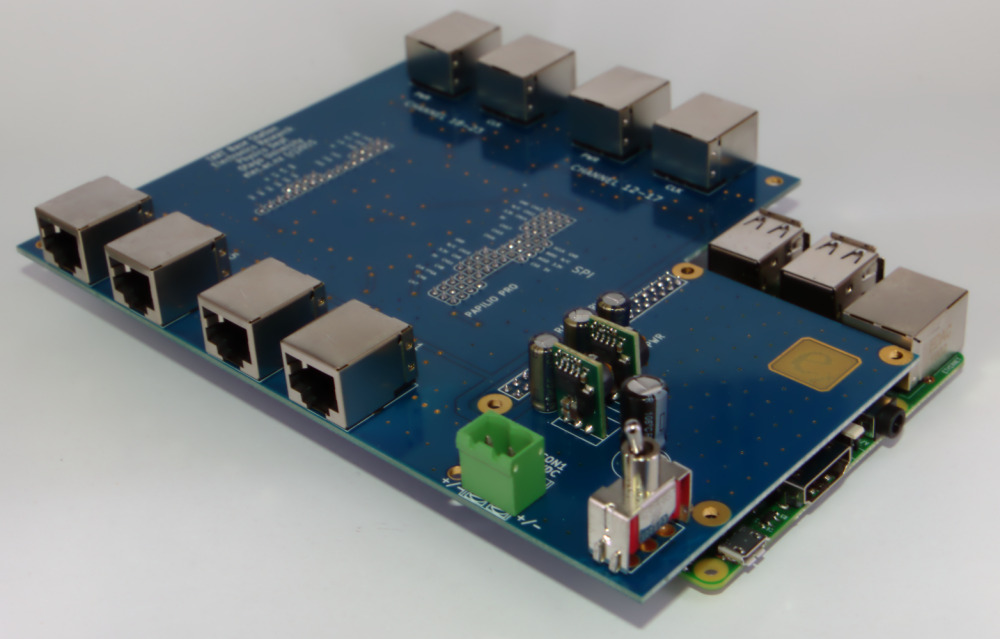
\includegraphics[height=0.4\textheight]{/home/tim/github/TART/doc/img/control_board_photo.png}
 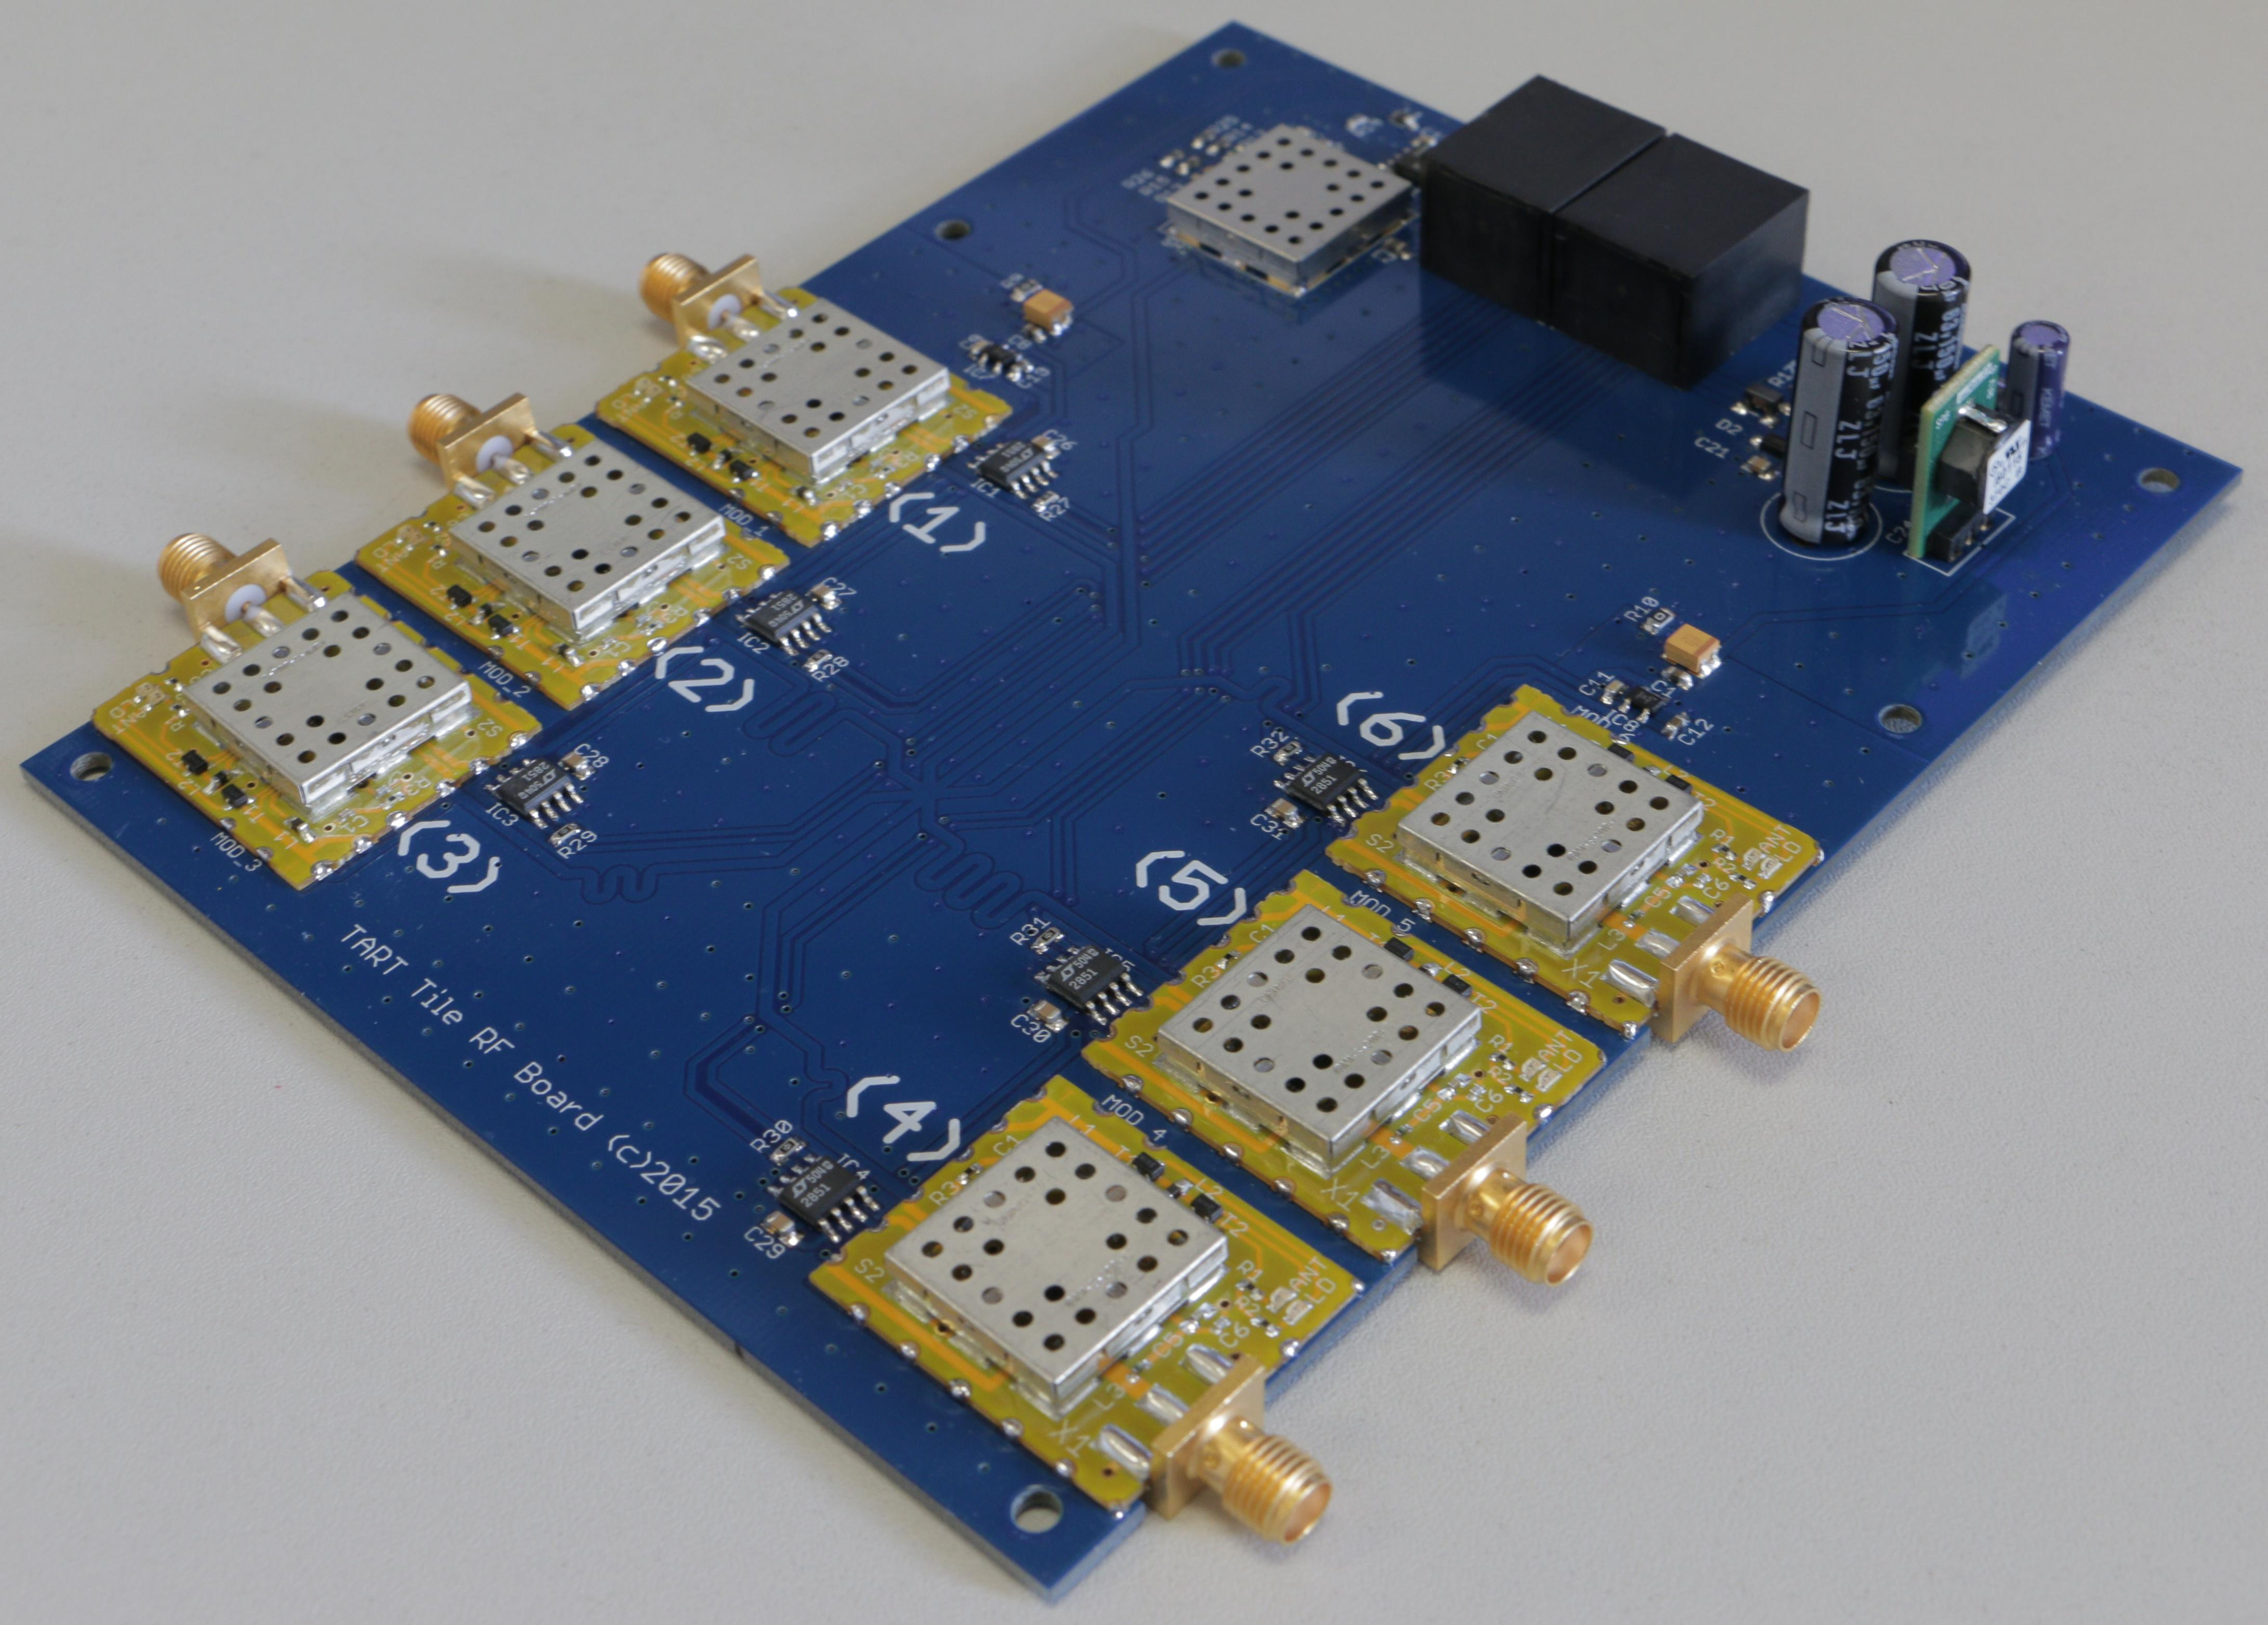
\includegraphics[height=0.4\textheight]{/home/tim/github/TART/doc/img/radio_hub_photo.jpg}

 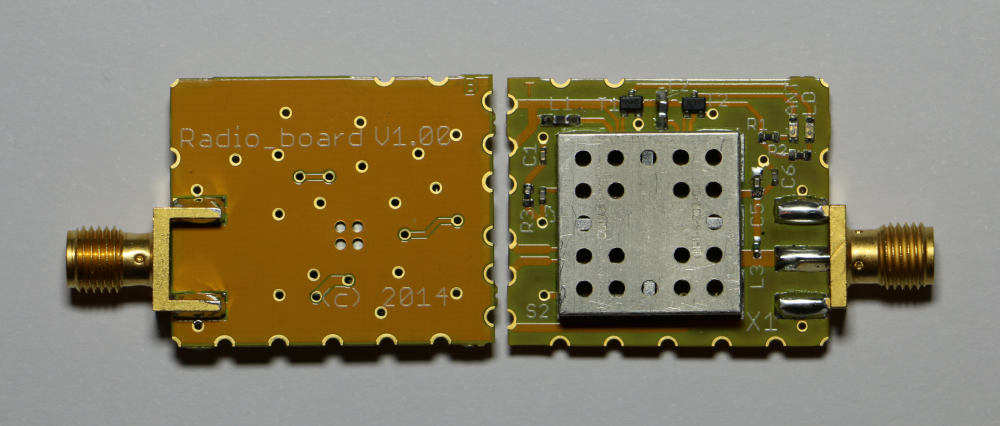
\includegraphics[width=0.7\linewidth]{/home/tim/github/TART/doc/img/radio_module.png}
\end{frame}

\begin{frame}{TART-2 Array}
 \begin{columns}[T]
  \begin{column}{0.5\linewidth}
   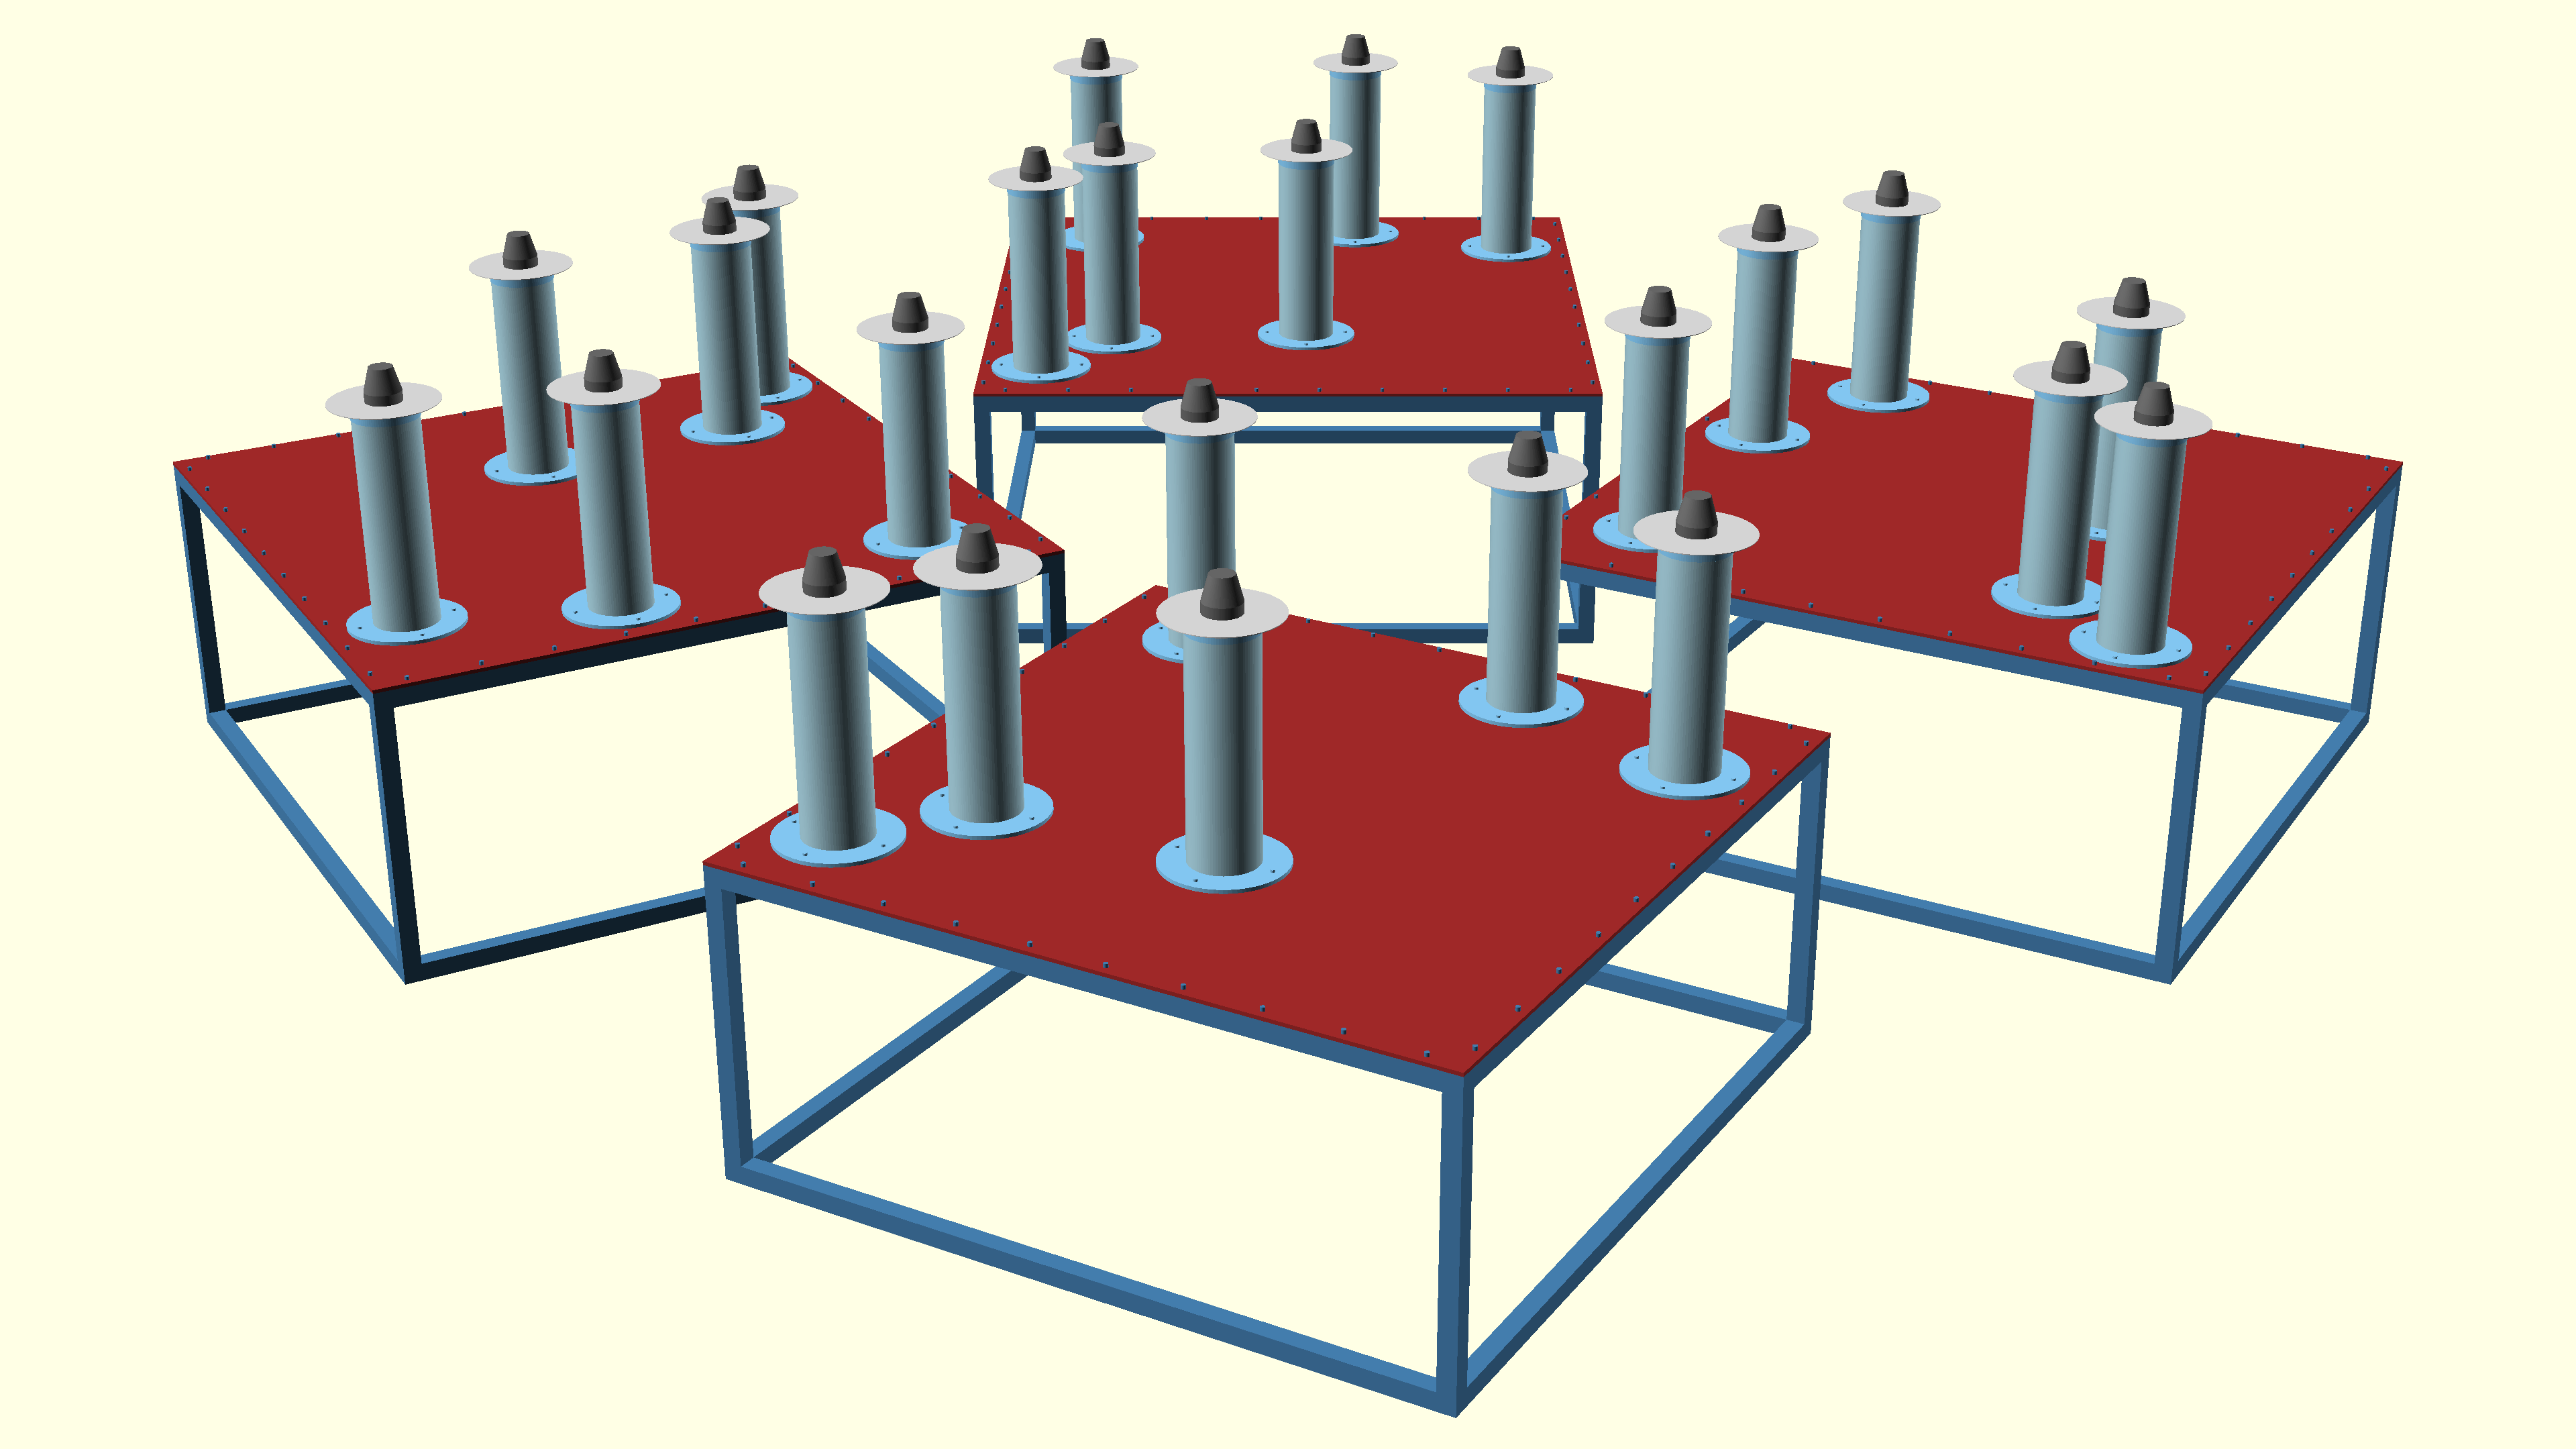
\includegraphics[width=\linewidth]{fig/tart2_array.png}
  Designed to optimize PSF sidelobes.
  \begin{itemize}
   \item Four identical tiles
   \item Easy to transport
  \end{itemize}
  \end{column}
  \begin{column}{0.5\linewidth}
  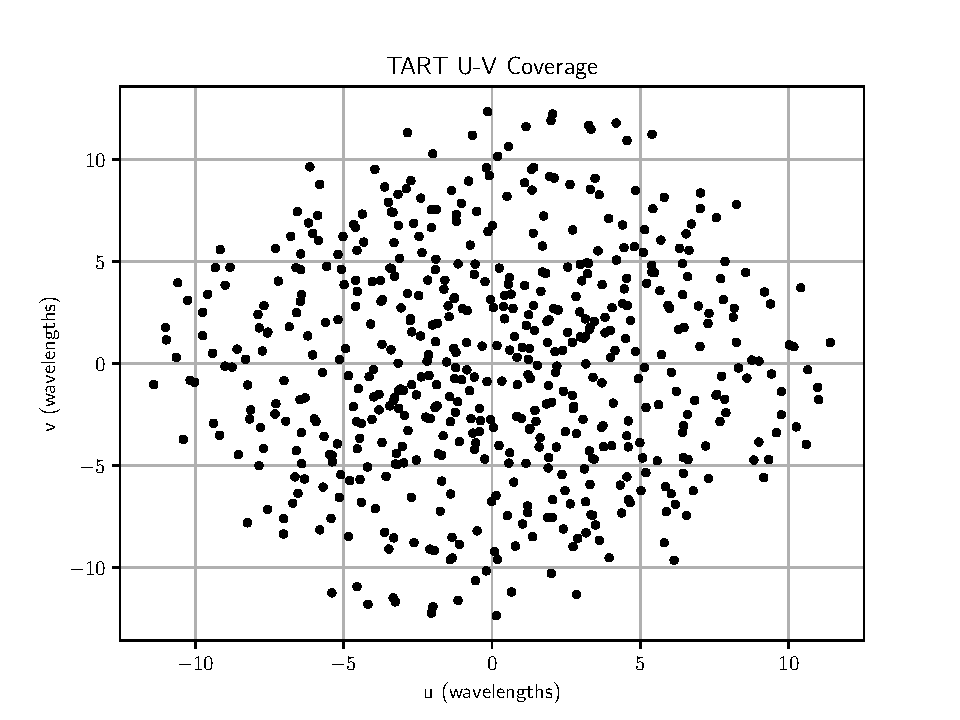
\includegraphics[width=\linewidth]{fig/TART_UV.pdf}
  \end{column}
 \end{columns}
\end{frame}

\begin{frame}{A better array design for TART-3}
 \includegraphics[width=\linewidth]{fig/five_arm_24.pdf}
 \begin{itemize}
  \item Easy to build
  \item Easy to change
  \item Good imaging properties.
 \end{itemize}

\end{frame}


\section{GRIME: The Gridded RIME}

\begin{frame}
\frametitle{Outline}
\tableofcontents[currentsection]
\end{frame}


\begin{frame}{GRIME Gridded RIME}
 Ignoring most things (antenna properties, polarization, co-ordinates e.t.c.):
 \begin{align}
      V_{ik} &= \iint S(\theta, \phi) e^{-2 \pi j (u_{ik} l + v_{ik} m + w_{ik}(n-1)} d \theta d \phi 
    \label{eqn:vis_theta_phi} 
    \equiv V(u_{ik}, v_{ik}, w_{ik}) 
 \end{align}
 \begin{columns}
  \begin{column}{0.5\linewidth}
   \begin{align*}
   l &= \sin(\phi) \cos(\theta) \\
    m &= \cos(\phi) \cos(\theta) \\
    n &= \sin(\theta)
  \end{align*}
  \end{column}
  \begin{column}{0.5\linewidth}
 \[ \vect{u} = \begin{pmatrix} u \\ v \\ w \end{pmatrix} \]   
  \end{column}
 \end{columns}
 This is an {\em inner product} in a Hilbert space 
 \[ V(u, v, w) = \left<S(\theta, \phi) \right| \left. H(u, v, w, \theta, \phi)\right > \]
\end{frame}

\begin{frame}{Discretizing the sky}
\begin{columns}
 \begin{column}{0.45\linewidth}
   Discretize $S(\theta, \phi)$ as a piecewise-constant function directly in angular coordinates. 
\begin{itemize}
\item The value of $s_k$, the $k$th element of the $\sky$, is the brightness of the {\em pixel} with $(\theta, \phi) = (\theta_k, \phi_k)$ and area $A_k$. 
 \item The sky $S(\theta, \phi)$ is 
represented as a vector, $\sky$ in an $N_s$ dimensional vector space $\skyspace$.
\item Can pixelize the entire sphere, or bits in any shape.
\end{itemize}
 \end{column}
 \begin{column}{0.55\linewidth}
 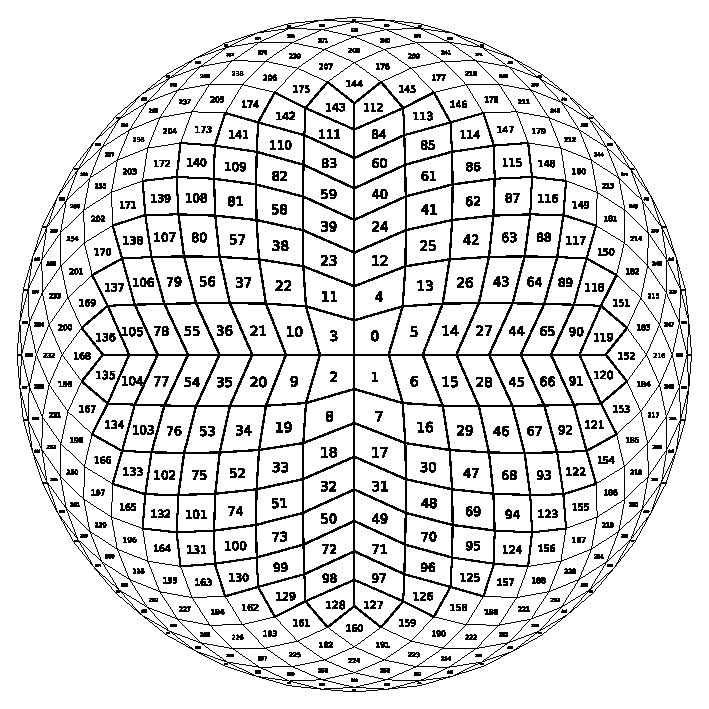
\includegraphics[width=\linewidth]{fig/hemisphere_pixels_3.pdf}  
 \end{column}
\end{columns}
\end{frame}

\begin{frame}{FFT Free Sky (FFS!)}

The expression for the visibility (Equation~\ref{eqn:vis_theta_phi}) in this representation is an inner-product in a finite vector space:
\begin{align}
 V(u, v, w) &= \sum_k^{N_s} A_k s_k e^{-2 \pi j (u l_k + v m_k + w(n_k-1)} \\ 
  &= \sky \cdot \fringe(u, v, w)
 \label{eqn:sky_fringe_vis}
\end{align}
$\fringe(u, v, w)$ is a vector in the sky space, which we refer to as an {\em fringe} vector. There is one fringe per visibility (baseline).
\end{frame}


\begin{frame}{Discrete Fringe Vectors}
 \begin{align}
  \fringe(u, v, w) &= \left( \begin{array}{c}
                A_1 e^{2 \pi j \left(u l_1 + v m_1 + (n_1-1) w \right)} \\
                A_2 e^{2 \pi j(u l_2 + v m_2 + (n_2-1) w )} \\
                A_3 e^{2 \pi j(u l_3 + v m_3 + (n_3-1) w )} \\
                 \vdots \\
                A_{N_s} e^{2 \pi j(u l_{N_s} + v m_{N_s} + (n_{N_s}-1) w )} \\
                \end{array} \right) \\
    &=\left( \begin{array}{c}
                 A_1\\
                 A_2 \\
                 A_3 \\
                 \vdots \\
                 A_k \end{array}  \right)  \odot \exp \left[ 2 \pi j \left( 
                    \begin{array}{c}
                 u l_1 + v m_1 + (n_1-1) w\\
                 u l_2 + v m_2 + (n_2-1) w \\
                 u l_3 + v m_3 + (n_3-1) w\\
                 \vdots \\
                 u l_{N_s} + v m_{N_s} + (n_{N_s}-1) w \\
                    \end{array}
                \right) \right] \nonumber \\
    &= \vect{a} \odot e^{2 \pi j \matr{B}\vect{u}}
    \label{eqn:fringe_vector}
\end{align}
\end{frame}

\begin{frame}
\begin{columns}
 \begin{column}{0.5\linewidth}
Choosing equal areas. Define:
\[
\fringe_i = \frac{1}{\sqrt{N_s}} e^{2 \pi j \matr{B} \vect{u_i}}
\]
Given a sky vector $\sky$, each baseline produces a visibility $V_i = \sky \cdot \fringe_i$, the dot-product of the sky vector with the associated fringe.
 \end{column}
 \begin{column}{0.5\linewidth}
\begin{center}
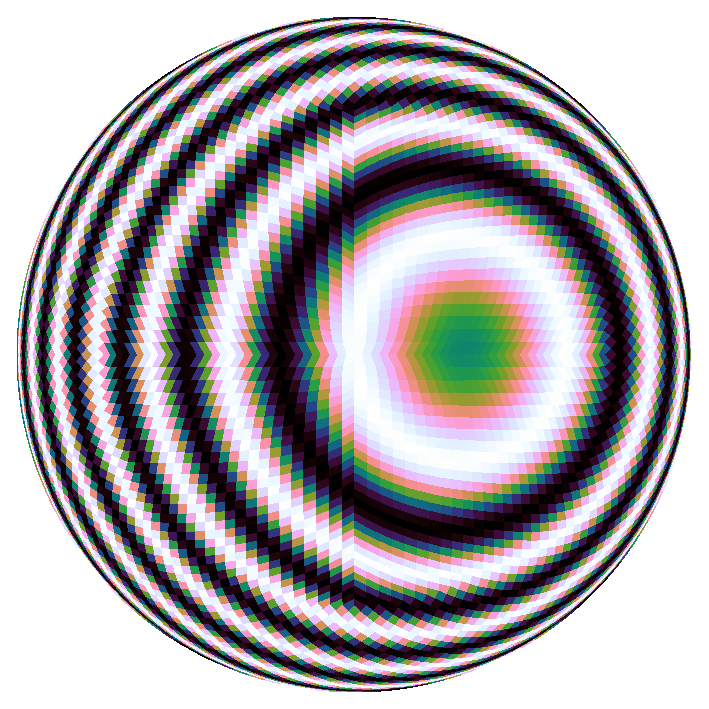
\includegraphics[width=0.45\linewidth]{fig/harmonic_uvw_0.pdf}
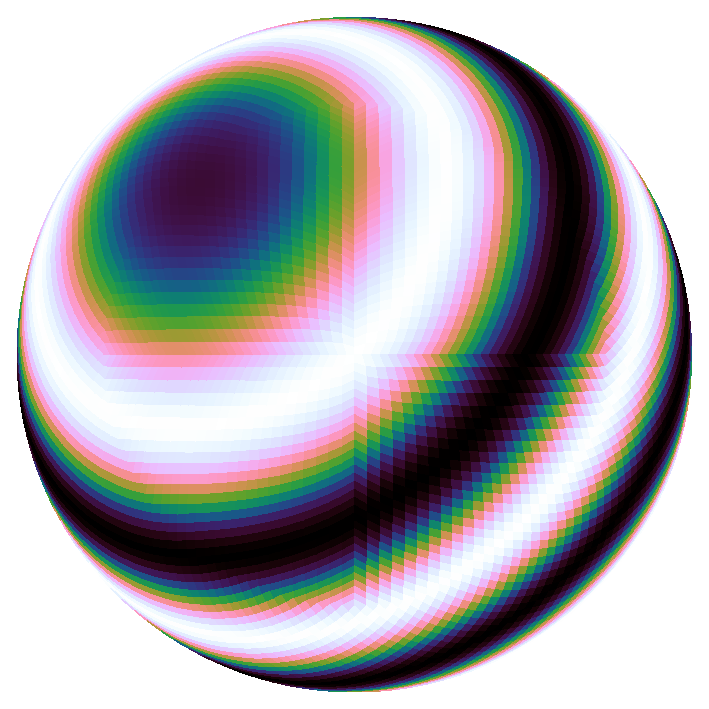
\includegraphics[width=0.45\linewidth]{fig/harmonic_uvw_1.pdf}\\
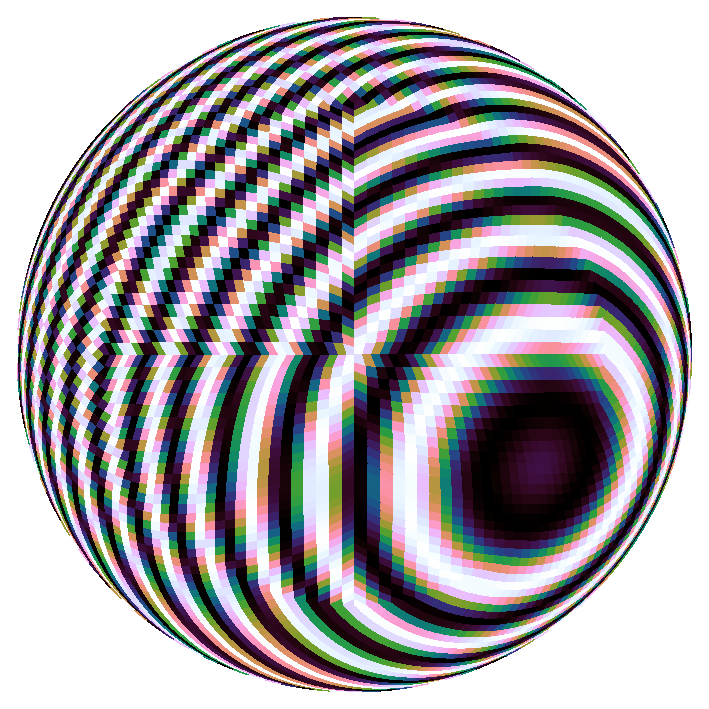
\includegraphics[width=0.45\linewidth]{fig/harmonic_uvw_2.pdf}
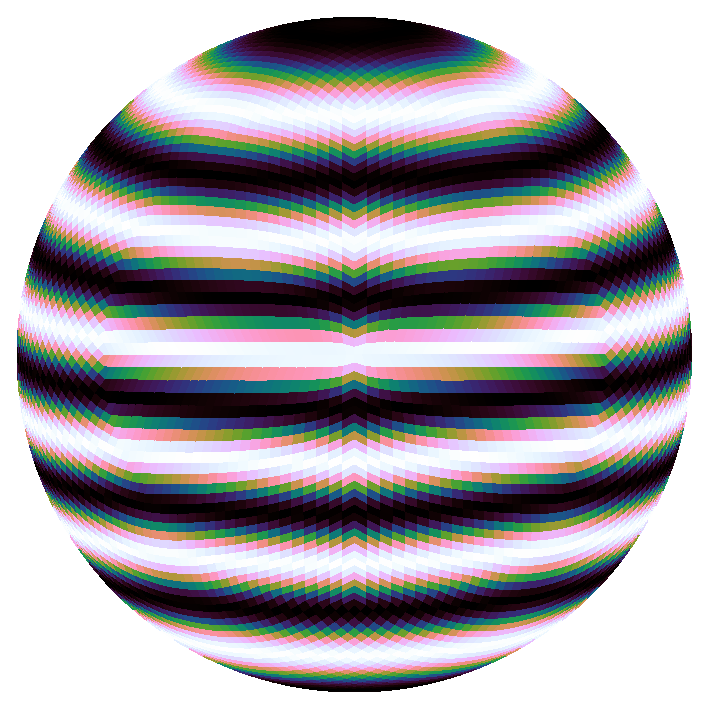
\includegraphics[width=0.45\linewidth]{fig/harmonic_uvw_3.pdf}
\end{center}  
 \end{column}
\end{columns}
\begin{block}{Note}
 Fringe vectors are sky vectors.
\end{block}
\end{frame}

% 
% 
% \begin{frame}{Properties of the Fringes}
% \begin{block}{Normalized}
%  Fringe vectors unit vectors. $\| \fringe_i \| = 1$.
% \end{block}
% \pause
% \begin{block}{Orthogonality}
% If fringe vectors were orthogonal, we could image by expressing the sky as a sum of fringe vectors.
% \begin{eqnarray*}
%  \sky = \sum_i^{N_v} V_i  \fringe_i & &
% S(l,m) = \iint V(u.v) e^{j \ldots} dl dm
% \end{eqnarray*}
% \end{block}
% \pause
% \begin{block}{Orthogonality}
%  Fringe vectors are {\em not} orthogonal. $\fringe_i \cdot \fringe_j \neq 0$.
% \end{block}
% \end{frame}
% 
% \begin{frame}{Telescope forward-map}
% The $i$th baseline has a fringe vector $\fringe_i$, and given a sky-brightness vector, $\sky$, the corresponding visibility $V_i$ is given by 
% \begin{align}
%  V_i  &= \sky \cdot \fringe_i
% \end{align}
% This is the {\em forward-map} for the telescope. 
% 
% \begin{block}{Imaging}
% The purpose of an imaging algorithm is to calculate a sky-brightness vector $\sky$ from a set of measured visibilities $\{ V_i^m \}$.  This is an {\em inverse problem}.
% \end{block}
% \end{frame}
% 
% 
% \subsection{Imaging Discrete Skies}
% 
% \begin{frame}{Practical discretizations of the sky: HEALPix}
%  \begin{columns}[T]
%   \begin{column}{0.4\linewidth}
%   Requirements:
%    \begin{itemize}
%     \item Equal-area
%     \item Isolateral
%     \item Well understood
%    \end{itemize}
%    HEALPix fits the bill. 	Available in C, C++, Fortran90, IDL, Java and Python!
%   \end{column}
%   \begin{column}{0.6\linewidth}
%  \begin{center}
% 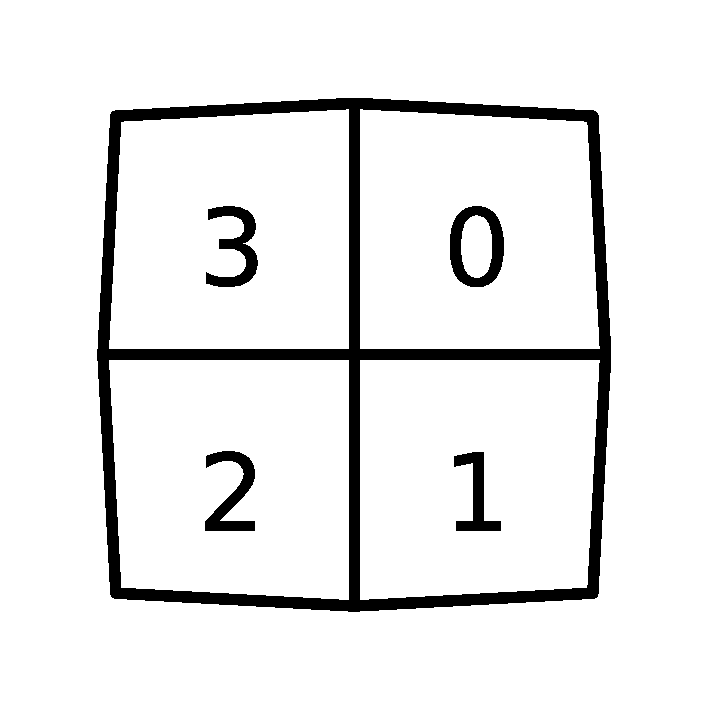
\includegraphics[width=0.45\linewidth]{fig/hemisphere_pixels_0.pdf}
% 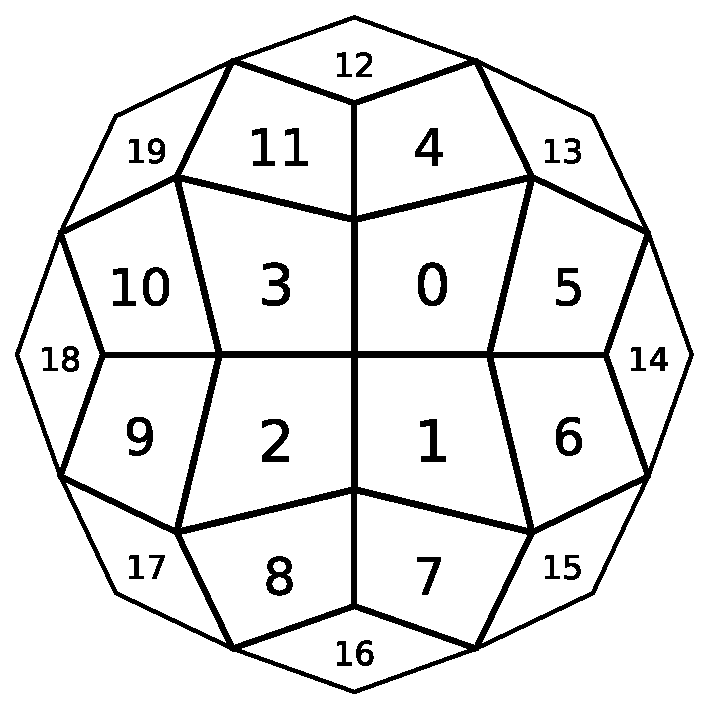
\includegraphics[width=0.45\linewidth]{fig/hemisphere_pixels_1.pdf}\\
% 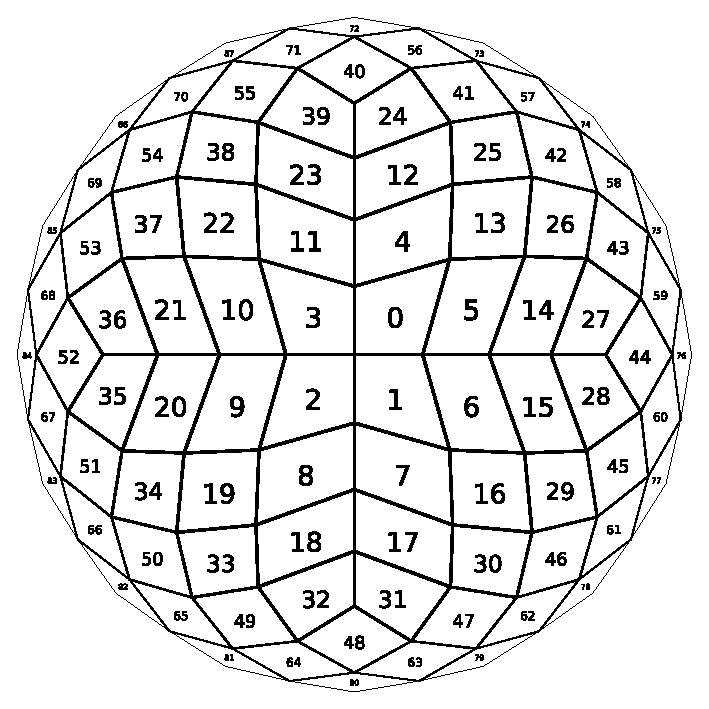
\includegraphics[width=0.45\linewidth]{fig/hemisphere_pixels_2.pdf}
% 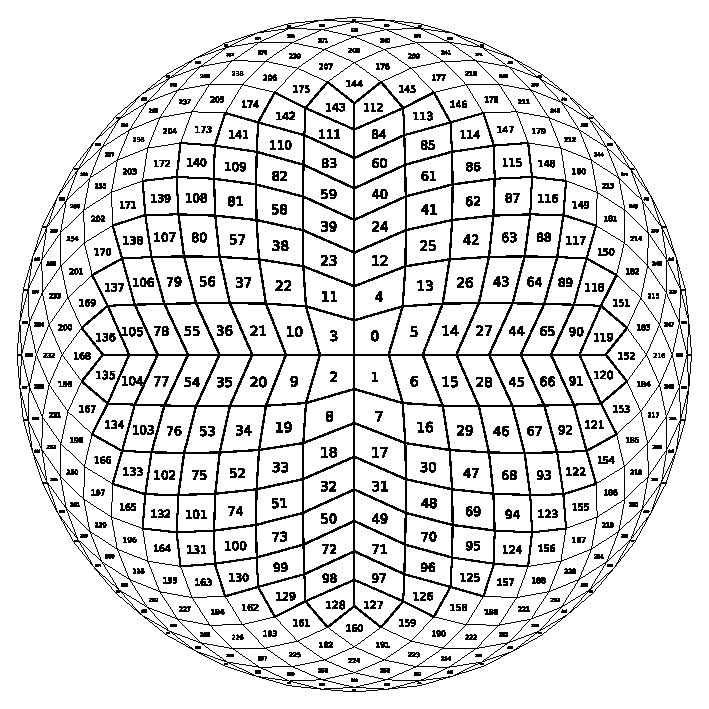
\includegraphics[width=0.45\linewidth]{fig/hemisphere_pixels_3.pdf}
% \end{center}   
%   \end{column}
%  \end{columns}
% \end{frame}
% 
% 
% %  \begin{columns}
% %   \begin{column}{0.3\linewidth}
% %   \end{column}
% %   \begin{column}{0.7\linewidth}
% %  \begin{center}
% % \end{center}   
% %   \end{column}
% %  \end{columns}
% 
% \subsection{Least-Squares}
% 
% \begin{frame}{Least-squares sky}
%  \begin{columns}
%   \begin{column}{0.35\linewidth}
%   Find $\vect{x} \in \skyspace$ that minimizes:
% \[ f(\vect{x}) = \sum_i^{N_v} \| V_i^m - \vect{x} \cdot \fringe_i \|^2 \]
% All-sky TART sky with $N_s = 12288$.
%   \end{column}
%   \begin{column}{0.65\linewidth}
%  \begin{center}
% \includegraphics[width=\linewidth]{{fig/disko_lsqr_2019_08_04_21_38_31_UTC}.pdf}
% \end{center}   
%   \end{column}
%  \end{columns}
% \end{frame}
% 

\subsection{\texorpdfstring{$L_1$}{L1} \& \texorpdfstring{$L_2$}{L2} Regularization}

% 2019-11-26 01:35:29,894 - disko.sphere - INFO - {'N_s':5568, 'S/N': 13.449562224969998, 'min': 0.0, 'max': 1.9007925330275814, 'mean': 0.07742980416164227, 'sdev': 0.1413274648819896, 'R_mad': 13.449562224969998, 'MAD': 0.1413274648819896, 'median': 0.0}

\begin{frame}{Tikhonov regularization 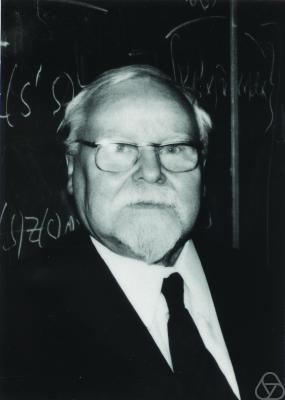
\includegraphics[width=0.25cm]{fig/Tychonoff.jpg}}
 \begin{columns}[T]
  \begin{column}{0.35\linewidth}
Find the sky, $\vect{x} \in \skyspace$, that minimizes
\[ f(\vect{x}) = \sum_i^{N_v} \| V_i^m - \vect{x} \cdot \fringe_i \|^2 + \alpha \| x \|^2 \]
\begin{itemize}
 \item Prefers a single sky solution (the shortest)
 \item Enforce positivity and reality.
 %  \foreignlanguage{russian}{Ти́хонов}
 \item Bayesian choice $\alpha = \frac{\sigma_v}{\sigma_0}$.
 \item Most probable if $\vect{x} = \normal(\vect{0}, \sigma_0 \matr{I})$ and $\vect{v} = \vect{v} +  \cnormal(\vect{0}, \sigma_v \matr{I})$.
\end{itemize}
  \end{column}
  \begin{column}{0.65\linewidth}
 \begin{center}
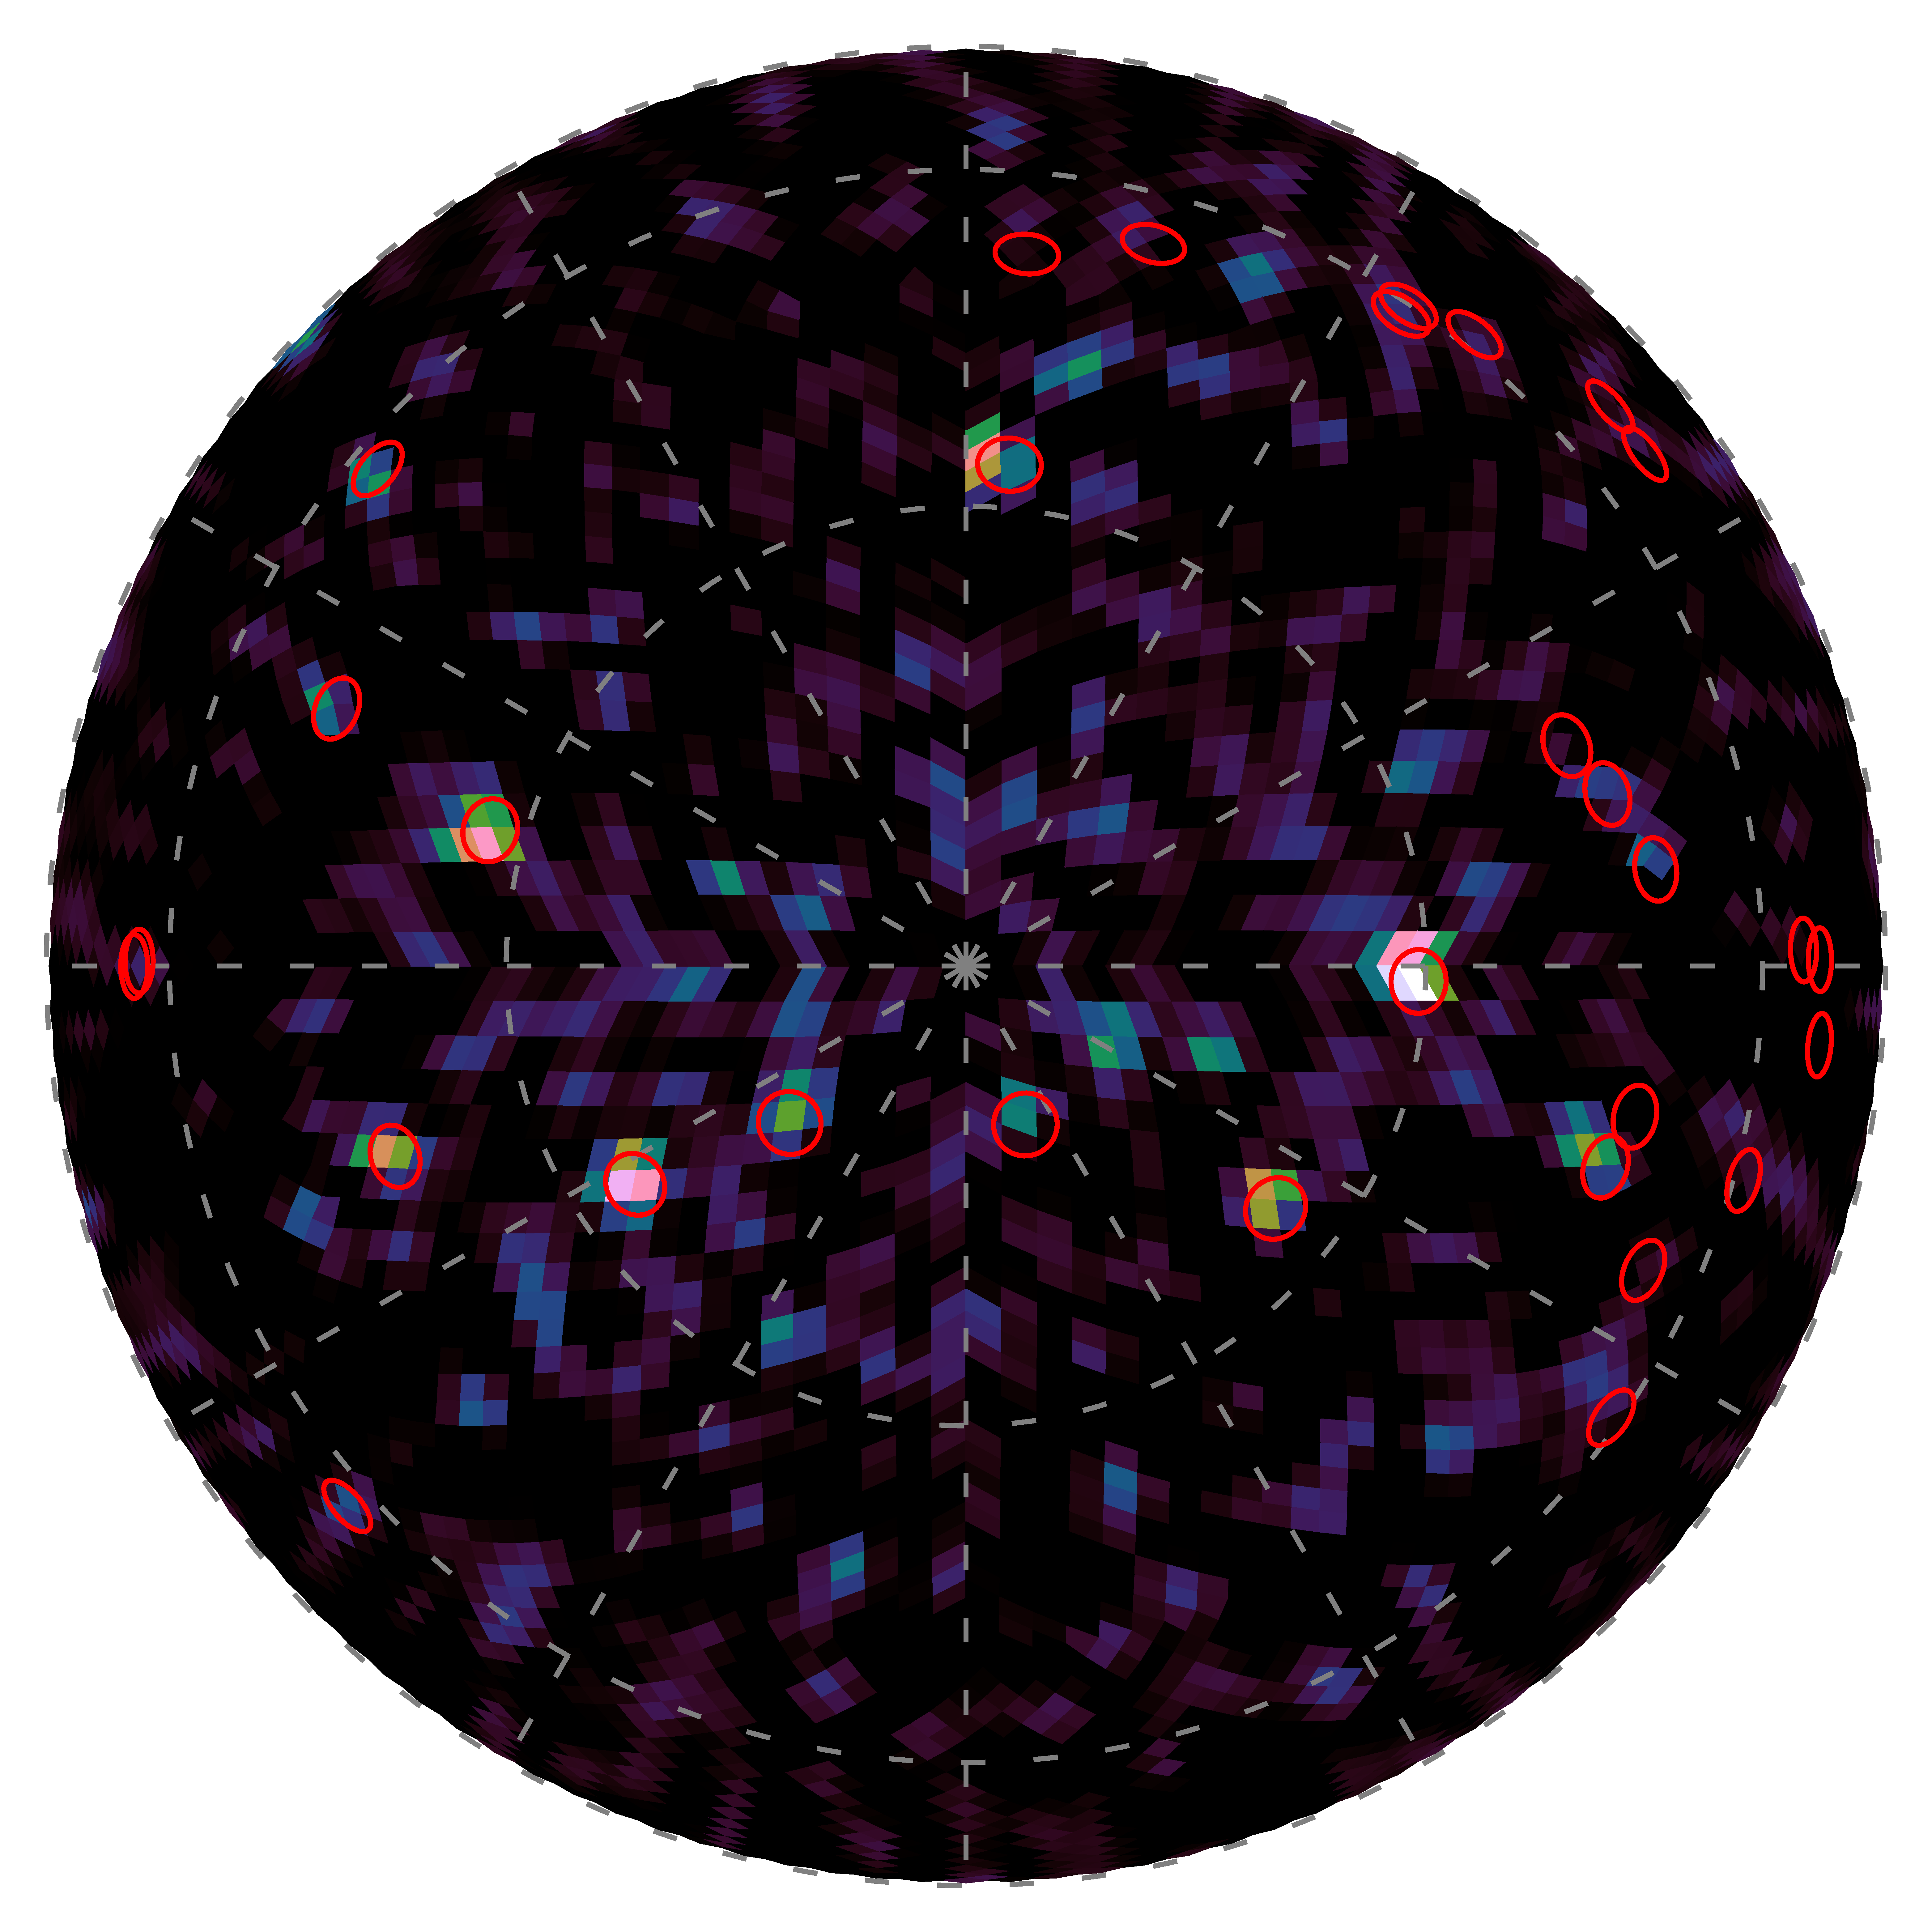
\includegraphics[width=\linewidth]{{fig/disko_tik_0.001_2019_08_04_21_38_31_UTC}.pdf}
\end{center}   
  \end{column}
 \end{columns}
\end{frame}




\begin{frame}{Lasso ($L_1$) regularization}
 \begin{columns}[T]
  \begin{column}{0.35\linewidth}
Find the sky, $\vect{x} \in \skyspace$, that minimizes
\[ f(\vect{x}) = \sum_i^{N_v} \left| V_i^m - \vect{x} \cdot \fringe_i \right| + \alpha \left| x \right| \]
\begin{itemize}
 \item Prefers sparsity (Fewest pixels)
 \item c.f. CLEAN
 \item Can enforce positivity and reality
 \item Optimum $\alpha$?
 \item Cross Validation
\end{itemize}
  \end{column}
  \begin{column}{0.65\linewidth}
 \begin{center}
   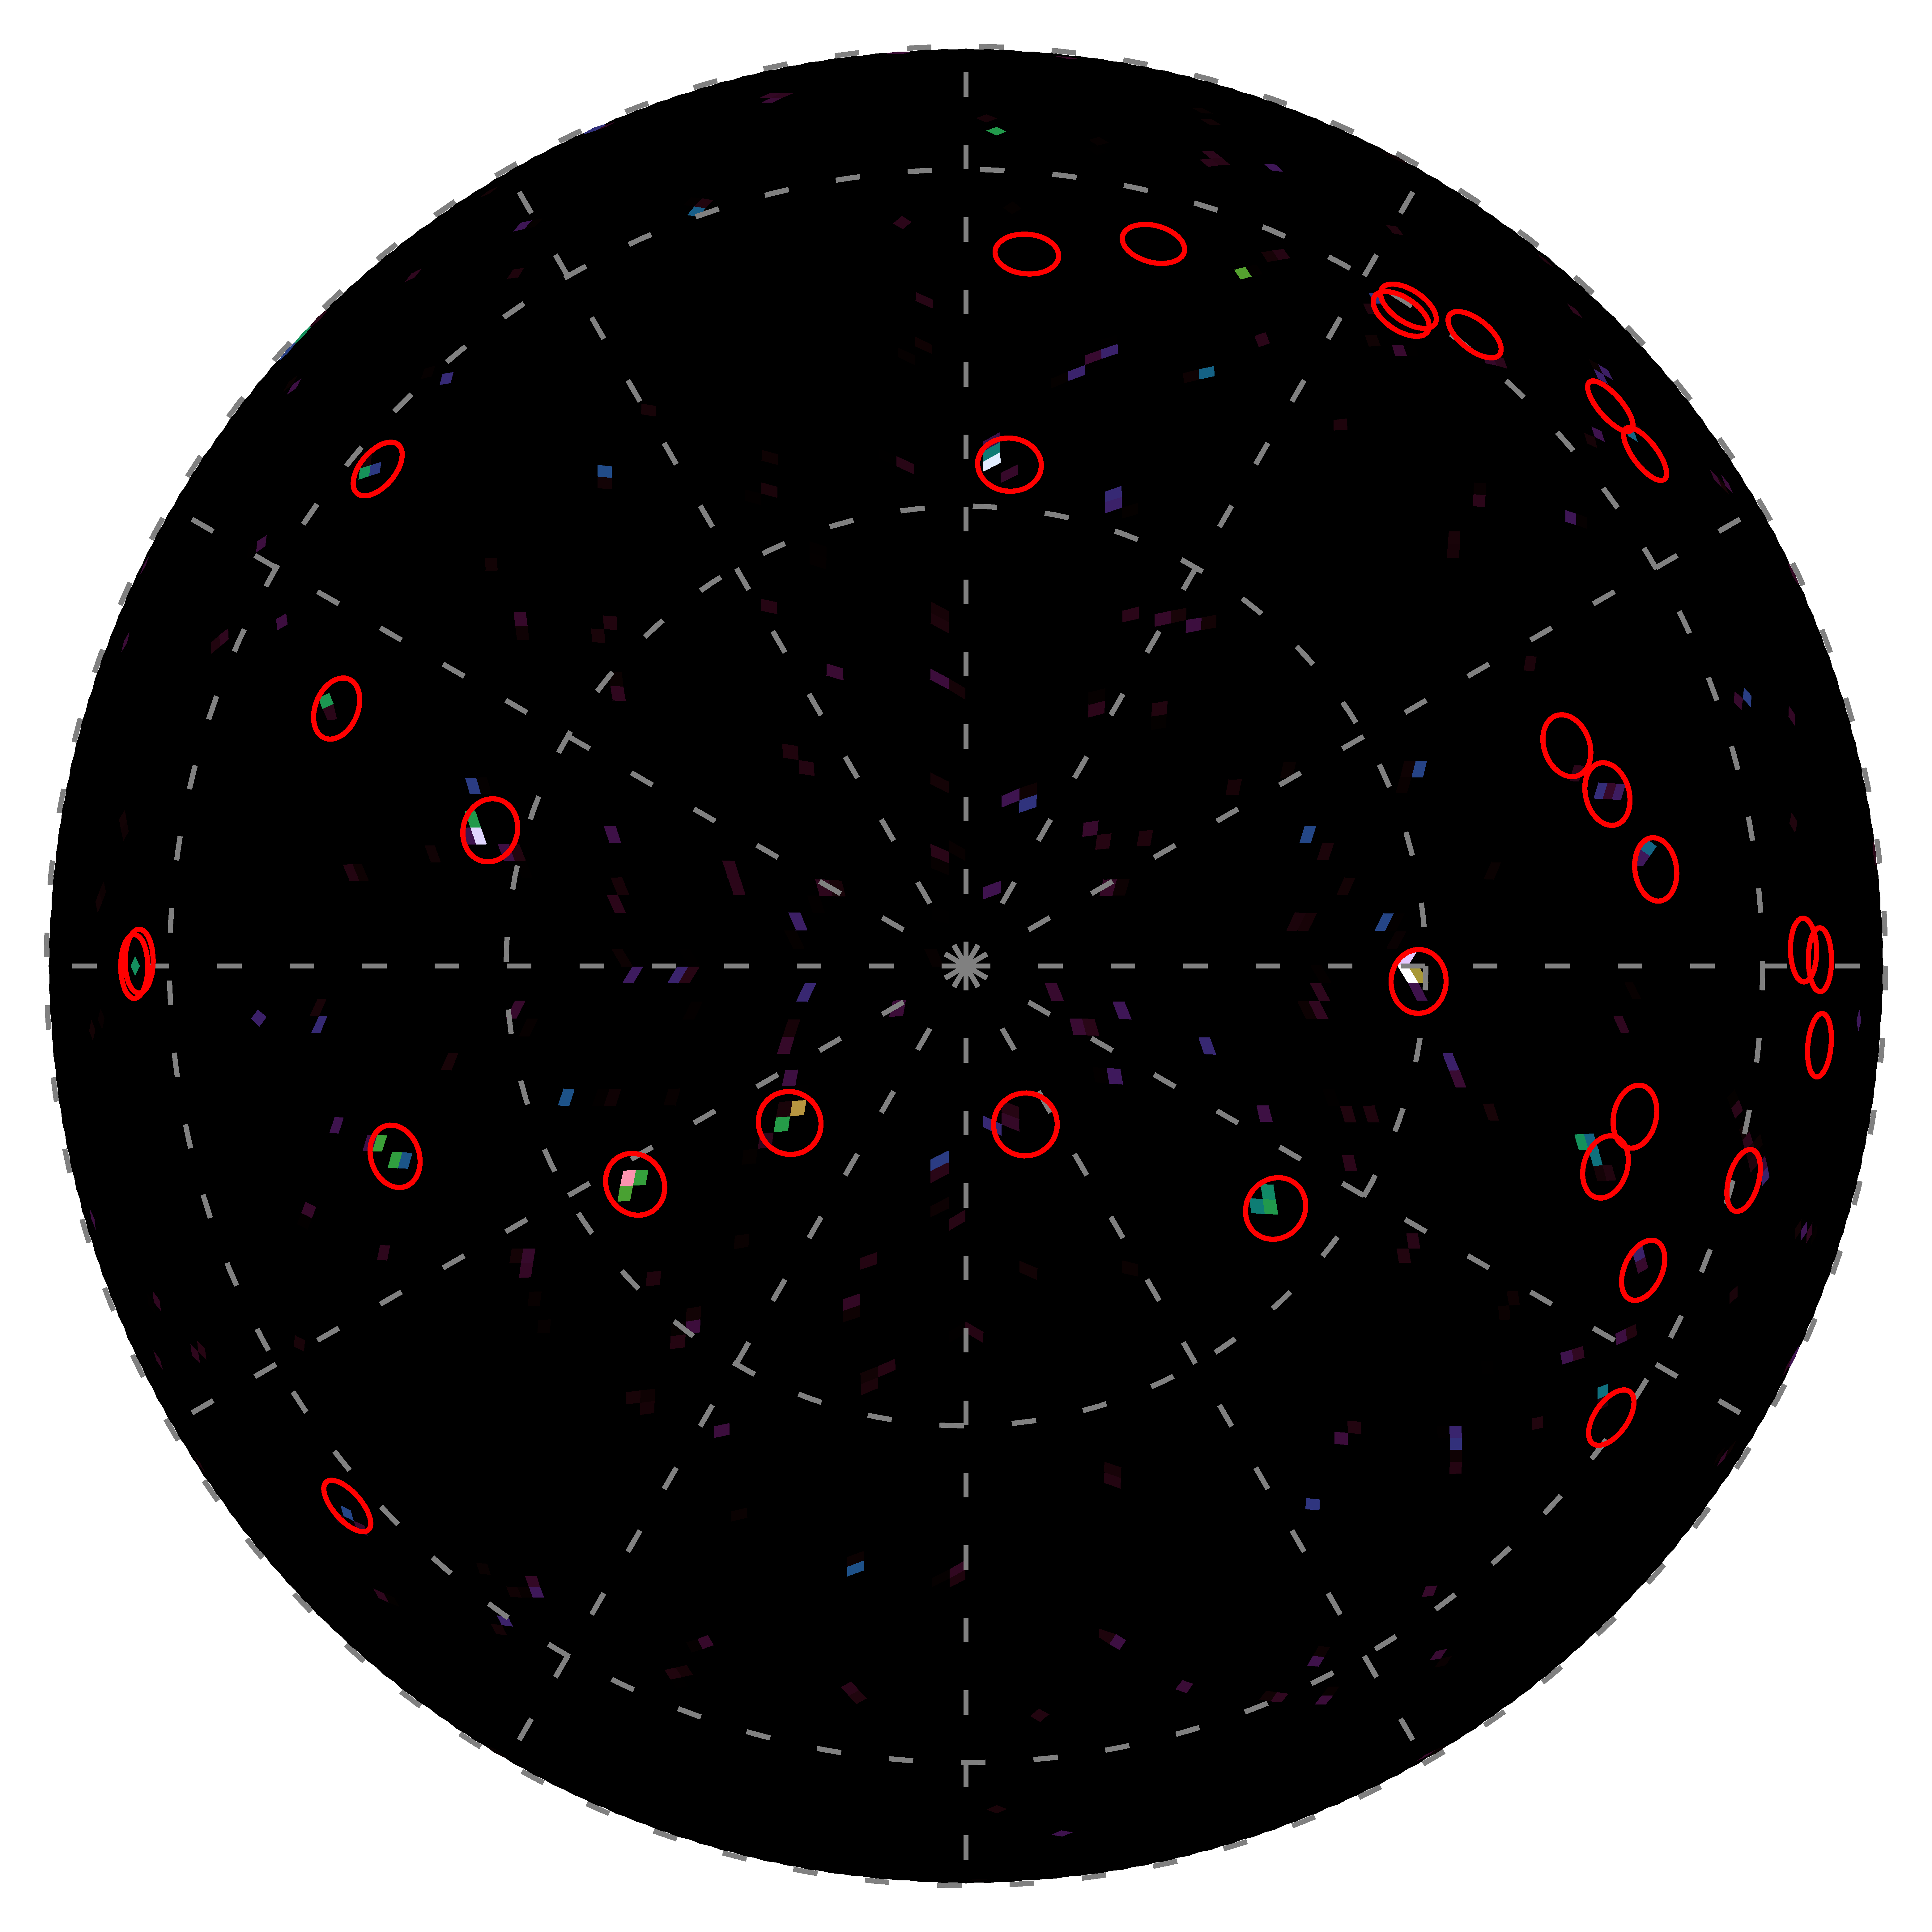
\includegraphics[width=\linewidth]{{fig/disko_2019_08_04_21_38_31_UTC}.pdf} 
\end{center}   
  \end{column}
 \end{columns}
\end{frame}
% 
% \begin{frame}{Round Images}
% \begin{columns}
%   \begin{column}{0.35\linewidth}
%    \begin{block}{The sky is not square}
% We have a framework for making any shape images we like.
% \end{block}
%    \begin{block}{What about primary beams?}
% Um, haven't got around to it yet.
% \end{block}
%   \end{column}
%   \begin{column}{0.65\linewidth}
%  \begin{center}
%    \includegraphics[width=\linewidth]{{fig/subsphere}.pdf} 
% \end{center}   
%   \end{column}
% \end{columns}
% \end{frame}
% 


\section{Matrix Formulation: The telescope operator}
\frame{\tableofcontents[currentsection]}


\begin{frame}{Matrix Form}
 Given an $N_v$ dimensional vector of visibilities $\mathbf{v}$, with one element for each baseline, the sky-vector, $\sky$, satisfies the equation,
\begin{equation}
\mathbf{v} = \gmat \sky
\label{eqn:telescope_operator_pixel_basis}
\end{equation}
Where $\gmat$ is the {\em telescope operator}, an $(N_v \times N_s)$ matrix with the fringes as row vectors. 

\[ T_{ik} = \frac{1}{\sqrt{N_s}} e^{j 2 \pi \left( u_i l_k  + v_i m_k + (n_i - 1) w_k \right)} \]
\begin{block}{Invertibility}
If $N_s > N_v$,  $\gmat$ is not invertible. The sky can not be uniquely determined from visibilities.
\end{block}

\end{frame}

% 
% \begin{frame}
% \begin{block}{Invertibility}
% If $N_s > N_v$,  $\gmat$ is not invertible. The sky can not be uniquely determined from visibilities.
% \end{block}
% From the rank-nullity theorem:
% \begin{itemize}
%  \item rank of $\gmat$ must be smaller than the number of baselines, i.e, $\rank(\gmat) \leq N_v$
%  \item the dimension of the space $\skyspace$ is $N_s$
%  \item null-space of $\gmat$ must be greater than $N_s - N_v$
% \end{itemize}
% Typically, $N_s \gtrsim  10^4$, and for TART, $N_v \sim 524$. The rank of the null-space is therefore far greater than the rank of the range space of $\gmat$. 
% \end{frame}

\begin{frame}{Approximate Inverse}

There is an approximate inverse:

 \[ s \sim \matr{T}^H \vect{v} \]
 
 Corresponds to the inverse FFT. Would be a solution if the $\fringe$ were actually orthogonal (or the sky were flat).
 
 \begin{block}{Could this be useful?}
  It might make a great preconditioner. As the equation
  \[ \matr{T}^H \vect{v} = \matr{T}^H \matr{T} \sky \]
  is sparse
 \end{block}
\end{frame}


\begin{frame}{Real Data: Cygnus}
 \begin{columns}[T]
  \begin{column}{0.4\linewidth}
github.com/tmolteno/disko
% 	/usr/bin/time -v disko --fov 0.3 --ms /home/tim/astro/cyg2052.ms --SVG --arcmin 0.2 --tikhonov --nvis 3000 --alpha 0.0025 --title 'cygnus'
\begin{itemize}
\item Tikhonov
\item 0.05 degree FOV
\item resolution 0.0007 is Nyquist
\item 230k pixels
\item 40k Visibilities
 \item 256 GB
\end{itemize}
  \end{column}
  \begin{column}{0.6\linewidth}
  \begin{center}
   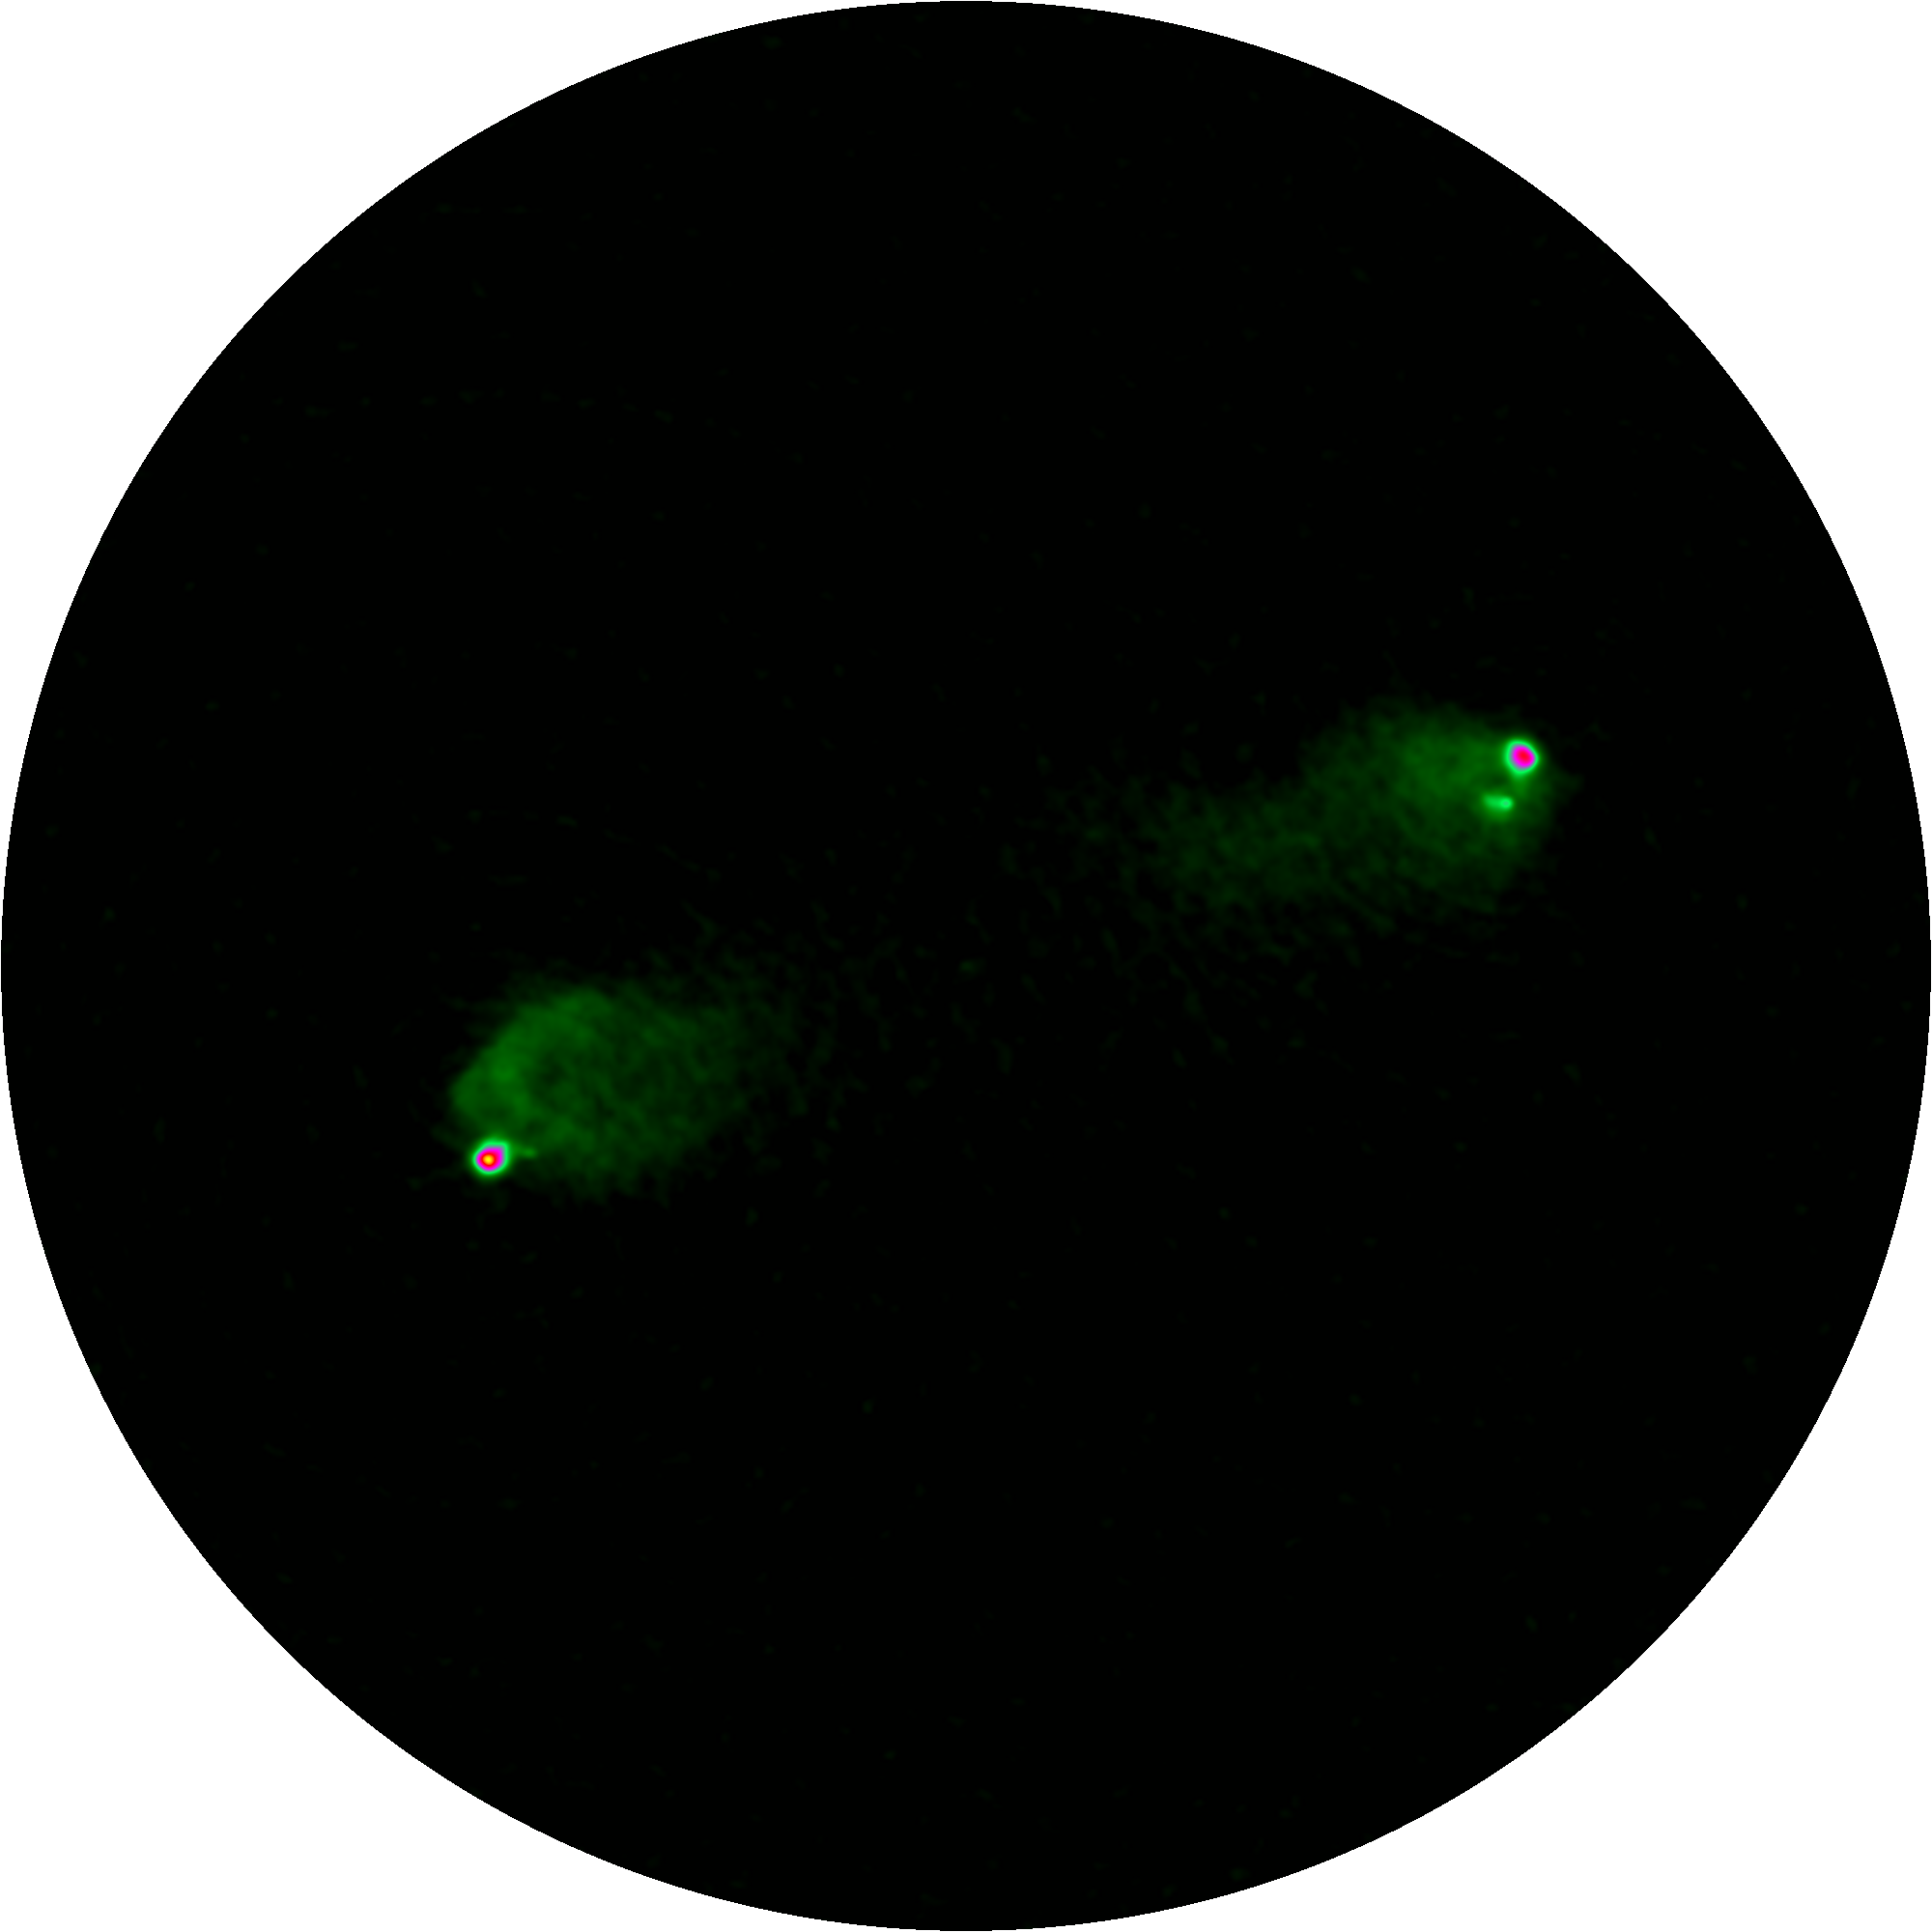
\includegraphics[width=\linewidth]{{fig/cygnus}.png} 
\end{center}     \end{column}
 \end{columns}
\end{frame}

\begin{frame}{1.5TB RAM}
 \begin{columns}[T]
  \begin{column}{0.4\linewidth}
MeerKAT data
% 	/usr/bin/time -v disko --fov 0.3 --ms /home/tim/astro/cyg2052.ms --SVG --arcmin 0.2 --tikhonov --nvis 3000 --alpha 0.0025 --title 'cygnus'
\begin{itemize}
\item 1.7 degree FOV
\item resolution 0.02 arcmin
\item 300k pixels
\item 30k Visibilities
 \item Still not enough resolution.
 \item Single frequency
\end{itemize}
  \end{column}
  \begin{column}{0.6\linewidth}
  \begin{center}
    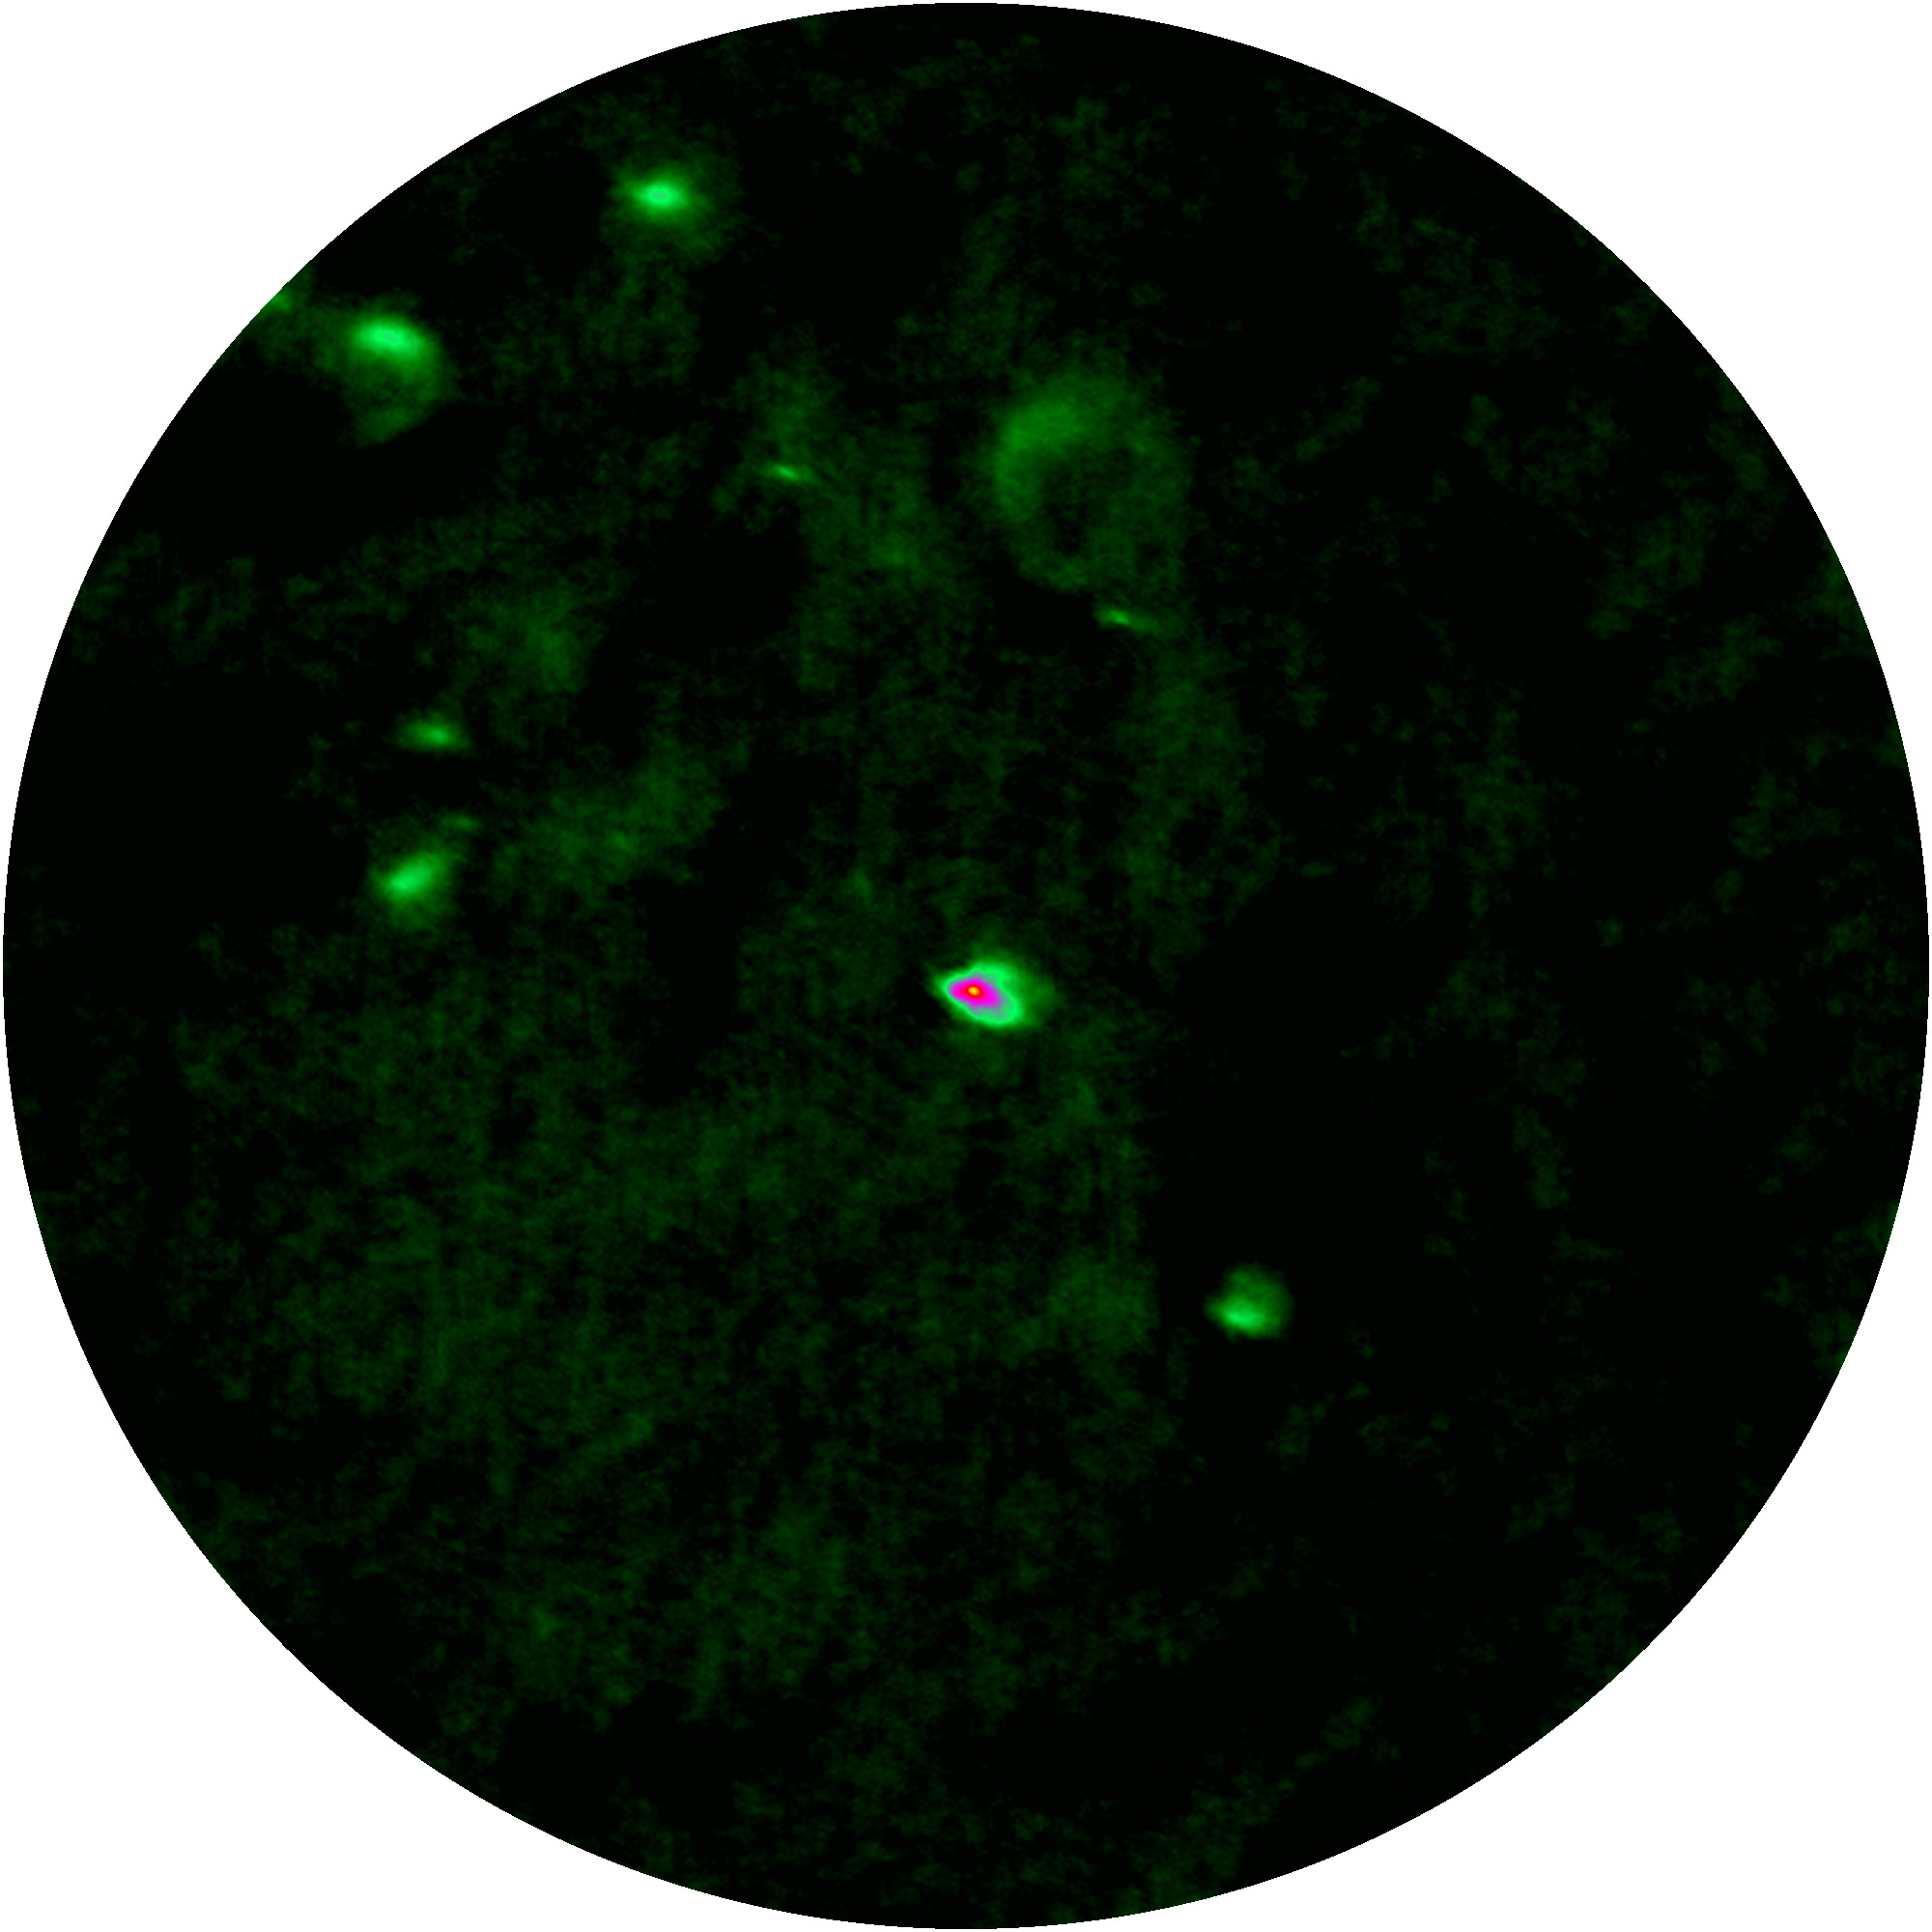
\includegraphics[width=\linewidth]{{fig/bubbles36k300k}.jpeg} 
\end{center}     
\end{column}
 \end{columns}
\end{frame}

% \begin{frame}{MeerKAT}
% For MeerKAT with $10^6$ pixels and $10^6$ visibilities:
% \begin{itemize}
%  \item RAM limits reached at $\sim 10^5 \times 10^5$ on AWS. 1.5 TB.
%  \item Matrix-free methods required
%  \item Conjugate Gradient with Preconditioner?
%  \item $\gmat^H$ is a bad preconditioner? (corresponds to steepest descent)
%  as $\gmat^H \gmat$ has double the condition number! (Fox)
%  \item Better to use an incomplete $LU$ decomposition?
% \end{itemize}
% \end{frame}
% 
% \begin{frame}{So far:}
% \begin{block}{Conclusion 1}
% Even a modest resolution discretized sky model is under-determined by snapshot visibility measurements.  Even on MeerKET with $N_V \sim 4000$.
% \end{block}
% \pause
% \begin{block}{Conclusion 2}
%  We've got a framework for making images of non-flat skies. Images can now be any shape (round, triangular, hexagonal, or anthing in between.\end{block}
% \pause
% \begin{block}{In the next part of this talk...}
% We'll pilfer standard linear operator results to characterize the {\em quality} of a telescope operator.
% \end{block}
% \end{frame}
% 
% 

\begin{frame}{Singular Value Decomposition}
 The telescope $\gmat$ is a map from sky vectors to visibility vectors. The SVD provides an explicit description of the range and null-space of this operator.
 \begin{align}
 \gmat &= \matr{U} \matr{\Sigma} \matr{V}^H  = 
        \begin{pmatrix}
             \matr{U_1} & \matr{U_2}
        \end{pmatrix} 
        \begin{pmatrix}
             \matr{\Sigma_1} & \matr{0} \\
             \matr{0} & \matr{0} \\
        \end{pmatrix} 
        \begin{pmatrix}
             \matr{V_1}^H \\ \matr{V_2}^H
        \end{pmatrix}
        \label{eqn:svd}
\end{align}
where:
\begin{itemize}
 \item $\matr{\Sigma_1} \in \real^{r \times r}$, 
 \item $\matr{U_1} \in \complex^{N_v \times r}$, $ \matr{U_2} \in \complex^{N_v \times (N_v - r)}$
 \item $\matr{V_1} \in \complex^{N_s \times r}$, $ \matr{V_2} \in \complex^{N_s \times (N_v - r)}$, 
 \item $r = \rank(\gmat)$.
\end{itemize}
\end{frame}

\begin{frame}{Batcave projected with $ \matr{P_n}$ into the null-space}
This image can be added to {\em any} TART image, and the result will be consistent with observations.
\begin{center}
 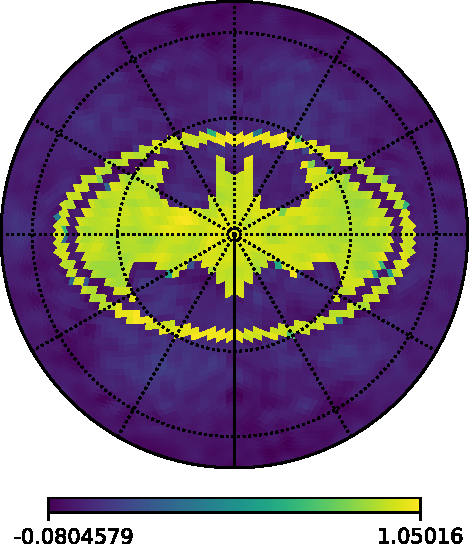
\includegraphics[width=0.6\linewidth]{fig/null_space_batman.pdf}
\end{center}
\end{frame}



\begin{frame}{Spectrum of TART}
  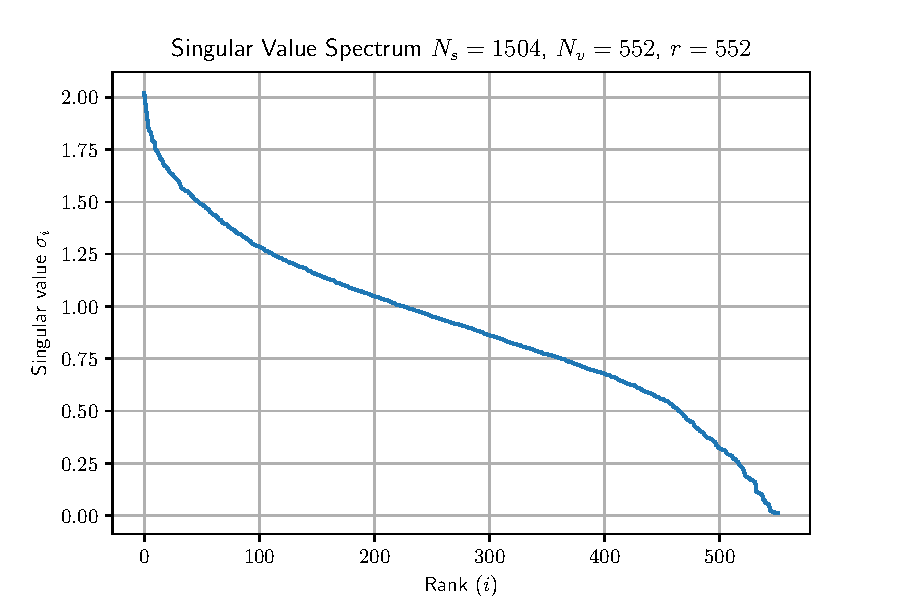
\includegraphics[width=\linewidth]{fig/TART_Singular_Ns_1504_Nv_552.pdf}
\end{frame}

% 
% \begin{frame}{SVD and Natural Basis}
% $\matr{V}^{H}$ transforms $\sky \in \skyspace$ into a new basis  factoring can easily be done
% \[ \vect{x} = \matr{V}^H \sky \] and as $\matr{V}$ is unitary $\sky = \matr{V}  \vect{x}$
% and therefore
% \begin{align}
%  \mathbf{v} &= \gmat \sky = \mathbf{U} \mathbf{\Sigma} \matr{V}^H \sky \\
%     &=  \mathbf{U} \mathbf{\Sigma}  \vect{x} = \matr{A} \vect{x} = \matr{A} (\vect{x_r} \oplus \vect{x_n}) = \matr{A} \vect{x_r}
% \end{align}
% Where $\matr{A} \equiv \matr{U} \matr{\Sigma}$ is the telescope operator in the natural basis for this telescope. The operator $\matr{A}$ has the form
% \[ \matr{A} = \begin{pmatrix}
%                \matr{A_r} & \matr{0}
%               \end{pmatrix} \]
% where $\matr{A_r}$ is an $r \times r$ square invertible matrix. In this case
% \begin{equation}
%  \vect{v} = \matr{A_r} \vect{x_r}
%  \label{eqn:natural_telescope_forward_map}
% \end{equation}
% This is the natural-basis telescope forward map.
% \end{frame}

\begin{frame}{Moore-Penrose Inverse}
 
As $\gmat$ has independent rows, the Moore-Penrose right-inverse, $\gmat^+$ is given by,
\[ \gmat^+ = \matr{V} \Sigma^+ \matr{U}^{*} \]
With $\gmat^+$ in hand, we can invert the telescope forward map as 
\[ \sky = \gmat^+ \mathbf{v} \]
This corresponds to the minimum L2-norm solution to the telescope equation.
% This is clearly closely related to using the inverse of $\matr{A_r}$ to retrieve the sky from the visibilities.
% \[ \vect{x_r} = \matr{A_r}^{-1} \vect{v} \]
\end{frame}

\section{Desigining Optimal Arrays}

\begin{frame}{Outline}
\tableofcontents[currentsection]
\end{frame}

\begin{frame}{Flat-sky (FFT-based) methods}
 \begin{quote}
  The point-source response is the Fourier Transform of the U-V coverage.
 \end{quote}
 Traditionally, the PSF of the telescope is calculated, and some heuristic is used like
 \begin{quote}
  Good U-V coverage.
 \end{quote}
 \begin{quote}
  Low-sidelobe levels in the synthesized beam.
 \end{quote}
 \begin{quote}
  Optimize the uniformity and spatial sensitivity.
 \end{quote}
 
\end{frame}

\begin{frame}{The Perfect Operator}
 The telescope operator is a function of the antenna spacings. The perfect operator:
 \begin{itemize}
  \item Has the maximum possible rank (reduces the dimension of the null-space)
  \item Reduces the posterior covariance (the volume in sky-probability space occupied by `images') as much as possible.
\item Is as insensitive to errors in antenna position as possible.
\end{itemize}

\end{frame}

\begin{frame}{SVD visualized}
 
\includegraphics[width=0.7\linewidth]{fig/svd.pdf}
\end{frame}

 
\begin{frame}{Pseudo-Condition number}

The {\em generalized condition number}~\cite{stanimirovic2001}, $K(\matr{T})$, of a matrix $\matr{T} \in C^{m \times n}_r$, is defined as
 \[ K(\matr{T}) = \lVert \matr{T} \rVert \lVert \matr{T}^+ \rVert \]

\begin{theorem}
If $\vect{v} = \matr{T} \sky$ is solvable, and $\sky = \matr{T}^+ \vect{v}$, and if $\sky + \delta \sky = \matr{T}^+( \vect{v}+ \delta \vect{v})$, then
 \[ \frac{\lVert \delta \sky \rVert}{\lVert \sky \rVert} \leq K(\matr{T}) \frac{\lVert \delta \vect{v} \rVert}{\lVert \vect{v} \rVert} \]
 \end{theorem}

 \begin{theorem}
If $\vect{v} = \matr{T} \sky$ is solvable, and $\sky = \matr{T}^+ \vect{v}$, and if $\sky + \delta \sky = (\matr{T} + \delta \matr{T})^+\vect{v}$, then
 \[ \frac{\lVert \delta \sky \rVert}{\lVert \sky \rVert} \leq K(\matr{T}) \frac{\lVert \delta \matr{T} \rVert}{\lVert \matr{T} \rVert \left(1 - \lVert \matr{T}^+ \rVert \lVert \delta \matr{T} \rVert \right)} \]
 \end{theorem} 
\end{frame}

\begin{frame}{Condition Number \& SVD}
The pseudo-condition number, $K(\matr{T})$, is the ratio of the largest to the smallest non-zero singular value
 \[ K(\matr{T}) = \frac{\sigma_0}{\sigma_r} \]
 \begin{block}{SVD}
All we need is the SVD to calculate the condition number
 \end{block}
 \end{frame}

\begin{frame}{von Neumann Entropy}

Describes how much the operator shrinks the density of states.

The von Neumann entropy of a matrix is:
  \[ S = \sum_i -\sigma_i \ln(\sigma_i) \]
 \begin{block}{SVD}
All we need is the SVD to calculate the entropy
 \end{block}
 \end{frame}


\begin{frame}{Amazing little-known result} 
 The kind folk at Google/Baidu have recently done both the theory and implementation of auto-differentiating the SVD of a complex matrix 
 
 \begin{block}{Wow!}
 We can now calculate the derivatives of the $\sigma_i$ w.r.t the antenna positions!
 \end{block}
\pause
 \begin{block}{Tensorflow}
 Stochastic gradient descent (SGD) and friends, can be used to find the antenna positions that minimize functions that involve the $\sigma_i$.
 \end{block}

\end{frame}

\begin{frame}[fragile]{Tensorflow}
\begin{lstlisting}[language=Python, ]
    rows = []
    penalty = 1
    for i in range(num_ant):
        for j in range(i+1, num_ant):
            u,v,w = _x[i] - _x[j]
            duv = (u**2 + v**2 + w**2)
            penalty += penalize(duv, min_spacing)
            exponent = -p2j*tf.cast(u*l + v*m + w*n_minus_1, tf.complex128)
            h = tf.exp(exponent) * pixel_areas
            rows.append(h)
    
    gamma = tf.stack(rows, axis=0)

    s = tf.linalg.svd(gamma, full_matrices=False, compute_uv=False)

    entropy = -tf.math.reduce_sum(tf.math.log(s) * tf.math.reciprocal(s))
    cond = (s[0] / s[275])
\end{lstlisting}
\end{frame}


\section{Results}

\begin{frame}{Outline}
\tableofcontents[currentsection]
\end{frame}


\begin{frame}{TART-2 Array}
 \begin{columns}[T]
  \begin{column}{0.5\linewidth}
%   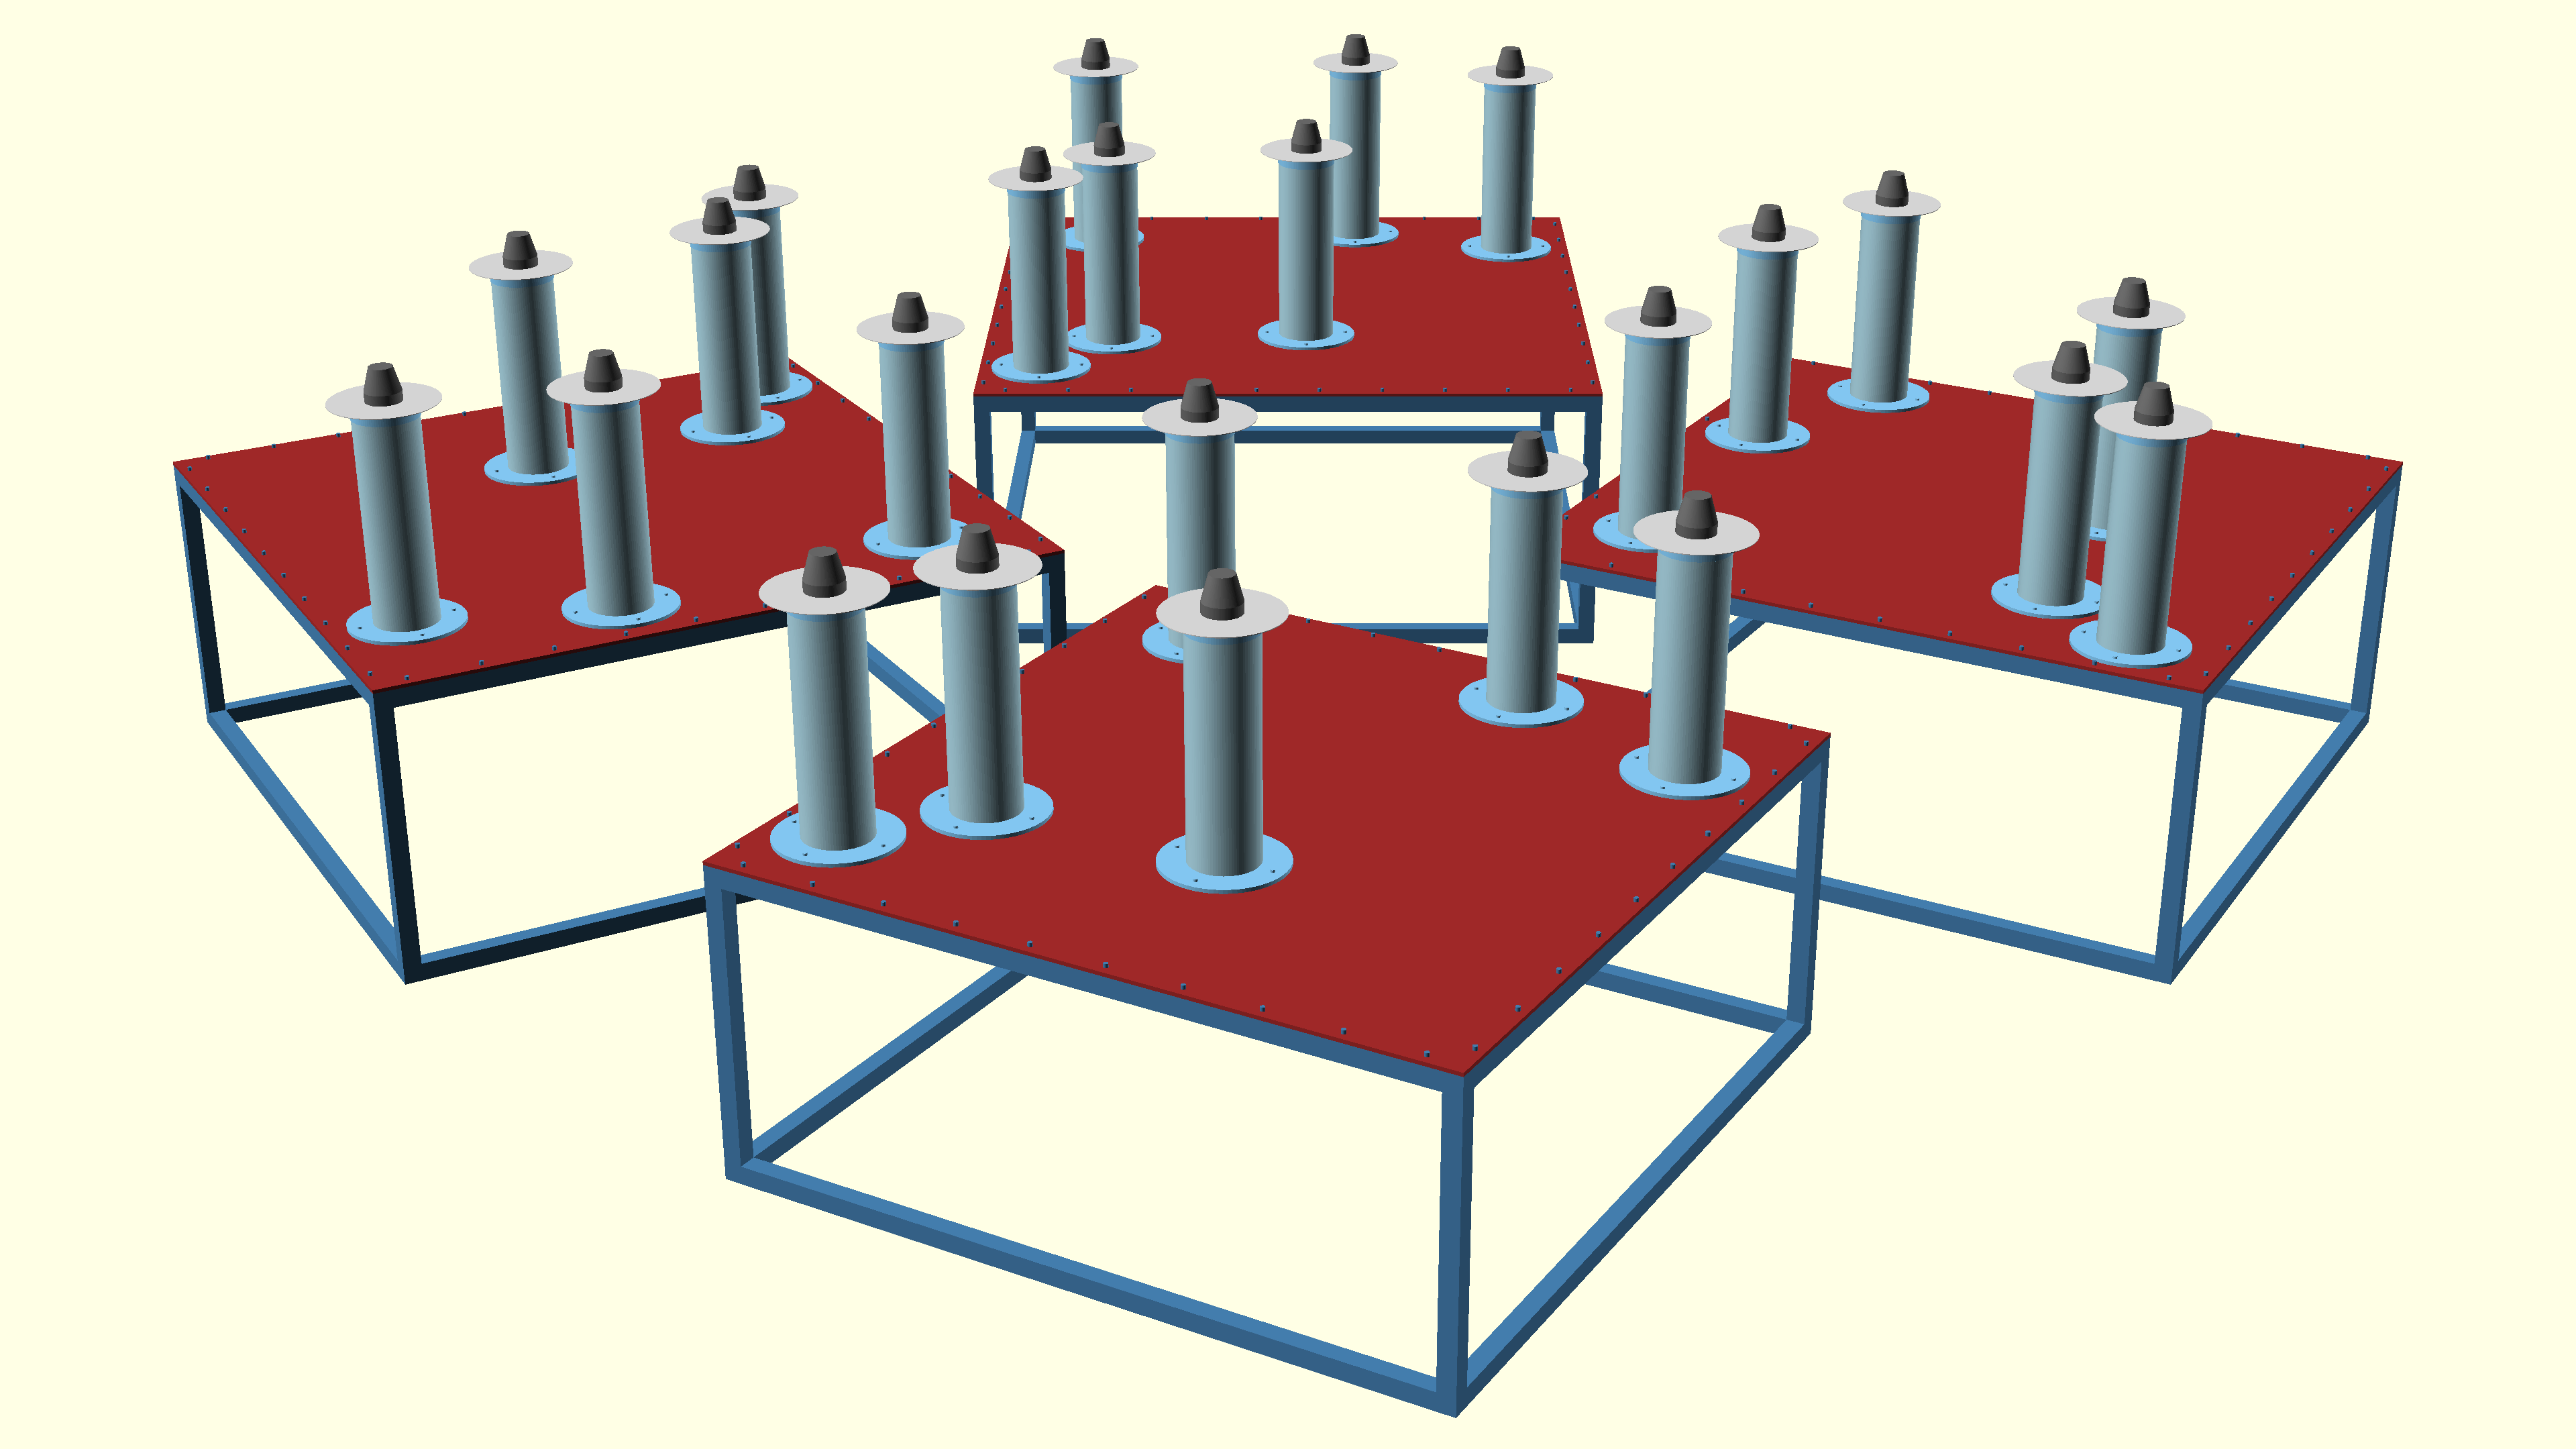
\includegraphics[width=\linewidth]{fig/tart2_array.png}
  Designed to optimize PSF sidelobes.
  \begin{itemize}
   \item Four identical tiles
   \item Easy to transport
  \end{itemize}
  \end{column}
  \begin{column}{0.5\linewidth}
  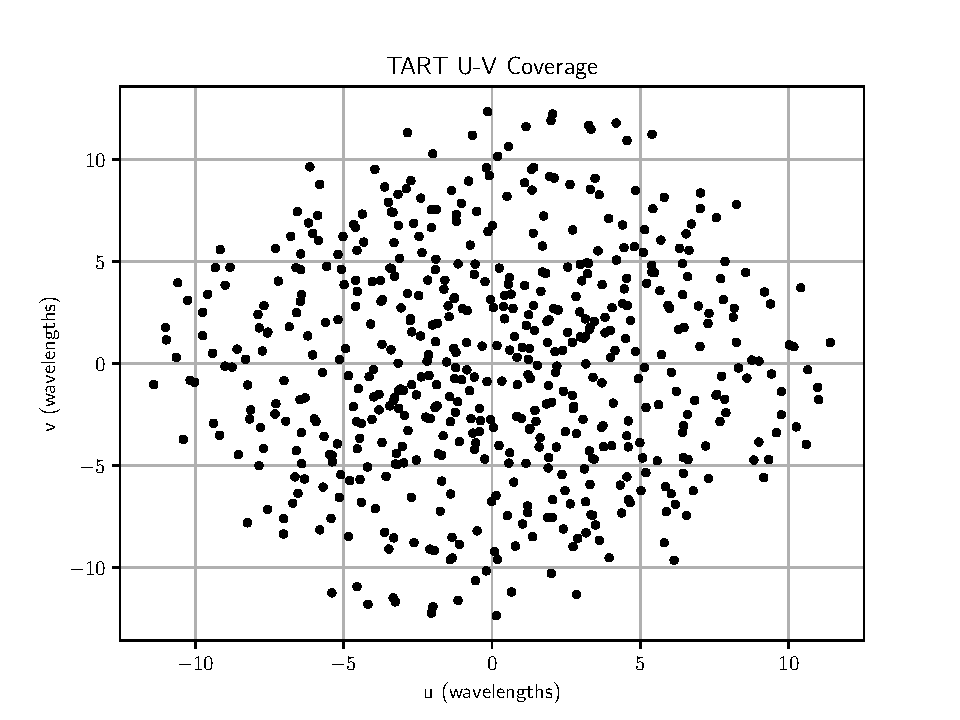
\includegraphics[width=\linewidth]{fig/TART_UV.pdf}
  \begin{itemize}
   \item $K(\matr{A}) = 188.2$
   \item Entropy: $S = 911.8$.
  \end{itemize}
  \end{column}
 \end{columns}
\end{frame}


\begin{frame}{Designing TART-3}
   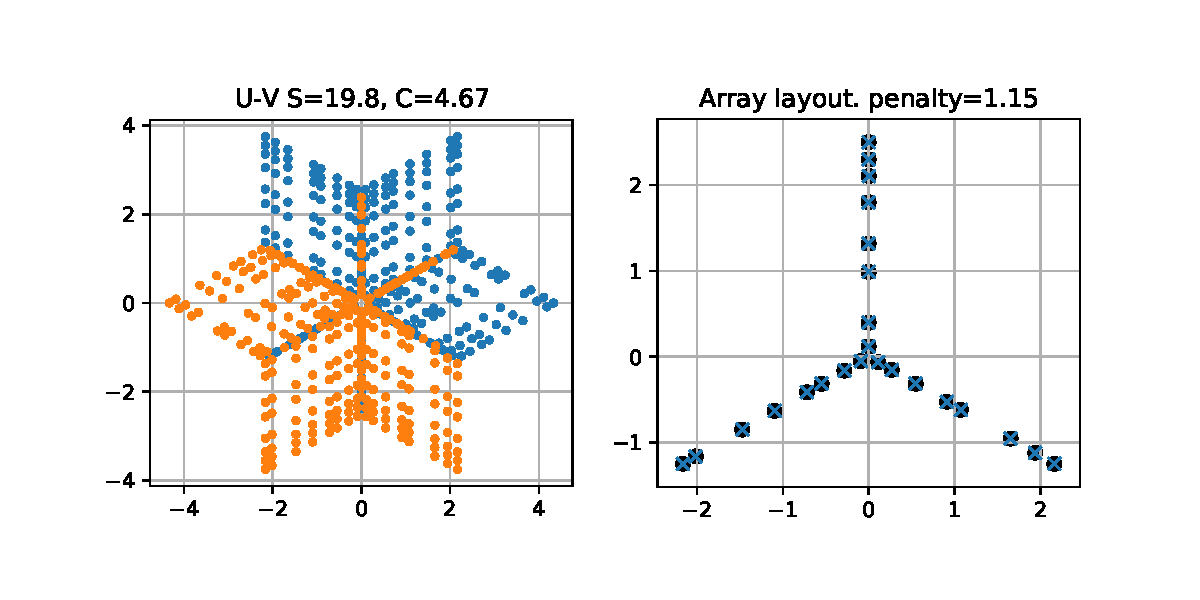
\includegraphics[width=\linewidth]{fig/optimum_tart_array.pdf}
 \begin{columns}
  \begin{column}{0.5\linewidth}
  \begin{itemize}
   \item The points aren't evenly spaced!
   \item Can be extended to earth-rotation synthesis.
  \end{itemize}
  \end{column}
  \begin{column}{0.5\linewidth}
  Penalty:
  \begin{itemize}
   \item Keeps antennas from overlapping
   \item Otherwise minimizing $K(A)$ involves overlap.
  \end{itemize}
  \end{column}
 \end{columns}

\end{frame}

\begin{frame}
    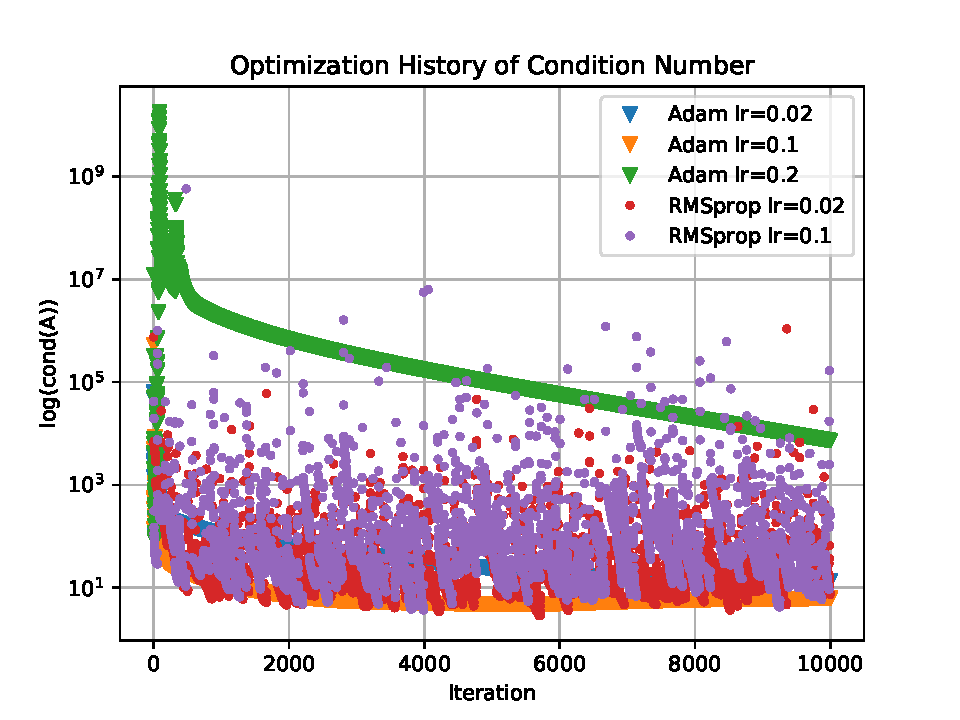
\includegraphics[width=\linewidth]{fig/optimization_history.pdf}
\end{frame}

\begin{frame}{Robustness}
How robust are the designs to errors in antenna position?
 \begin{columns}
  \begin{column}{0.5\linewidth}
  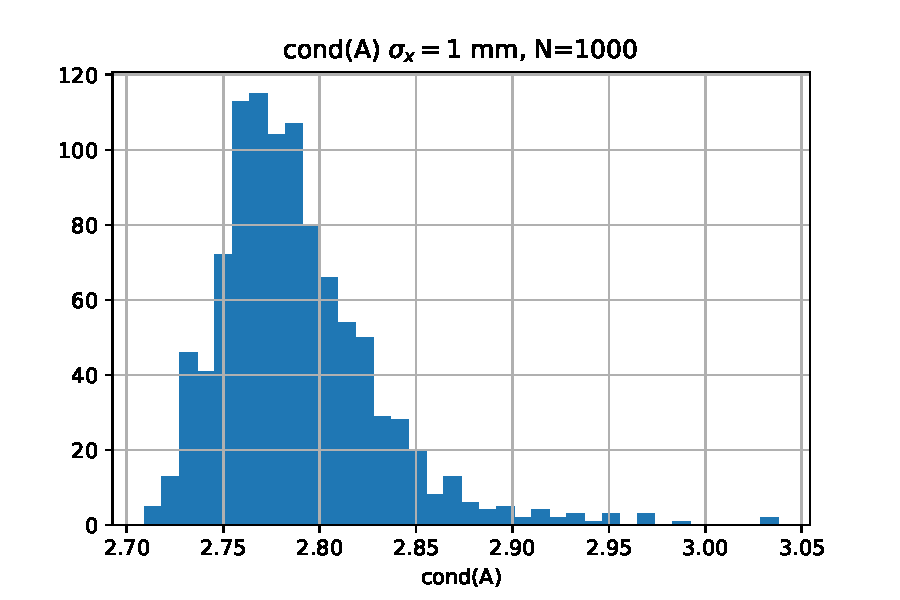
\includegraphics[width=\linewidth]{fig/cond_histogram.pdf}
  Adding random errors (1mm) to the antenna positions.
  \end{column}
  \begin{column}{0.5\linewidth}
  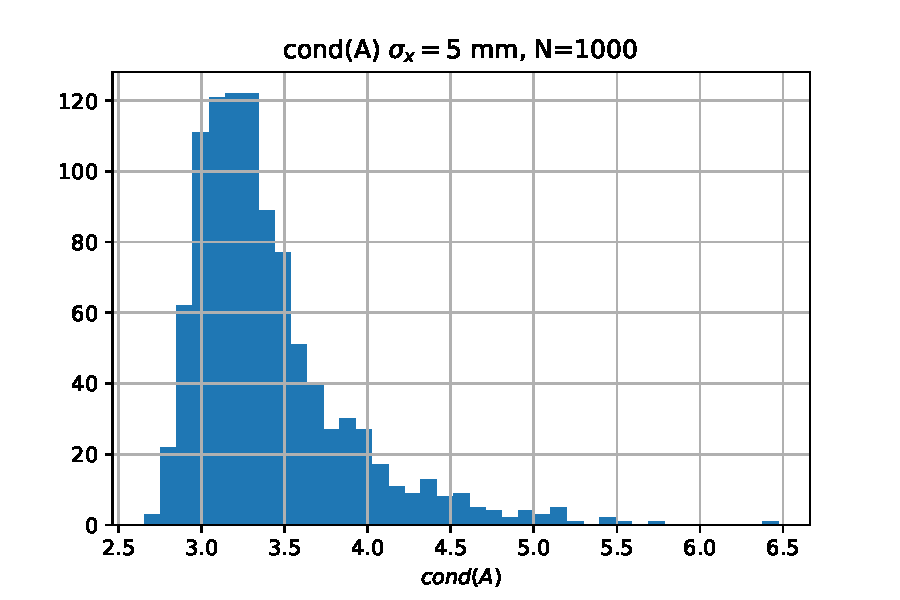
\includegraphics[width=\linewidth]{fig/cond_histogram5.pdf}   
  Adding random errors (5mm) to the antenna positions.
  \end{column}
 \end{columns}
 \begin{block}{Idea}
  If the condition number is minimized, then the array is maximally robust to antenna position errors. (The difference between expected and actual visibilities is minimized)
 \end{block}

\end{frame}

\begin{frame}{Discussion}

\begin{itemize}
 \item Seems to work!
 \item Computation scales very well (Tensorflow).
 \item $K(A)$ and $S$ mostly follow each other (but not always).
\end{itemize}

TODO:
\begin{itemize}
\item Are the Entropy/Cond designs any better?
\item How do existing arrays fare under these criteria?
\item Might be useful for future instruments. 
\end{itemize}
\end{frame}

\begin{frame}
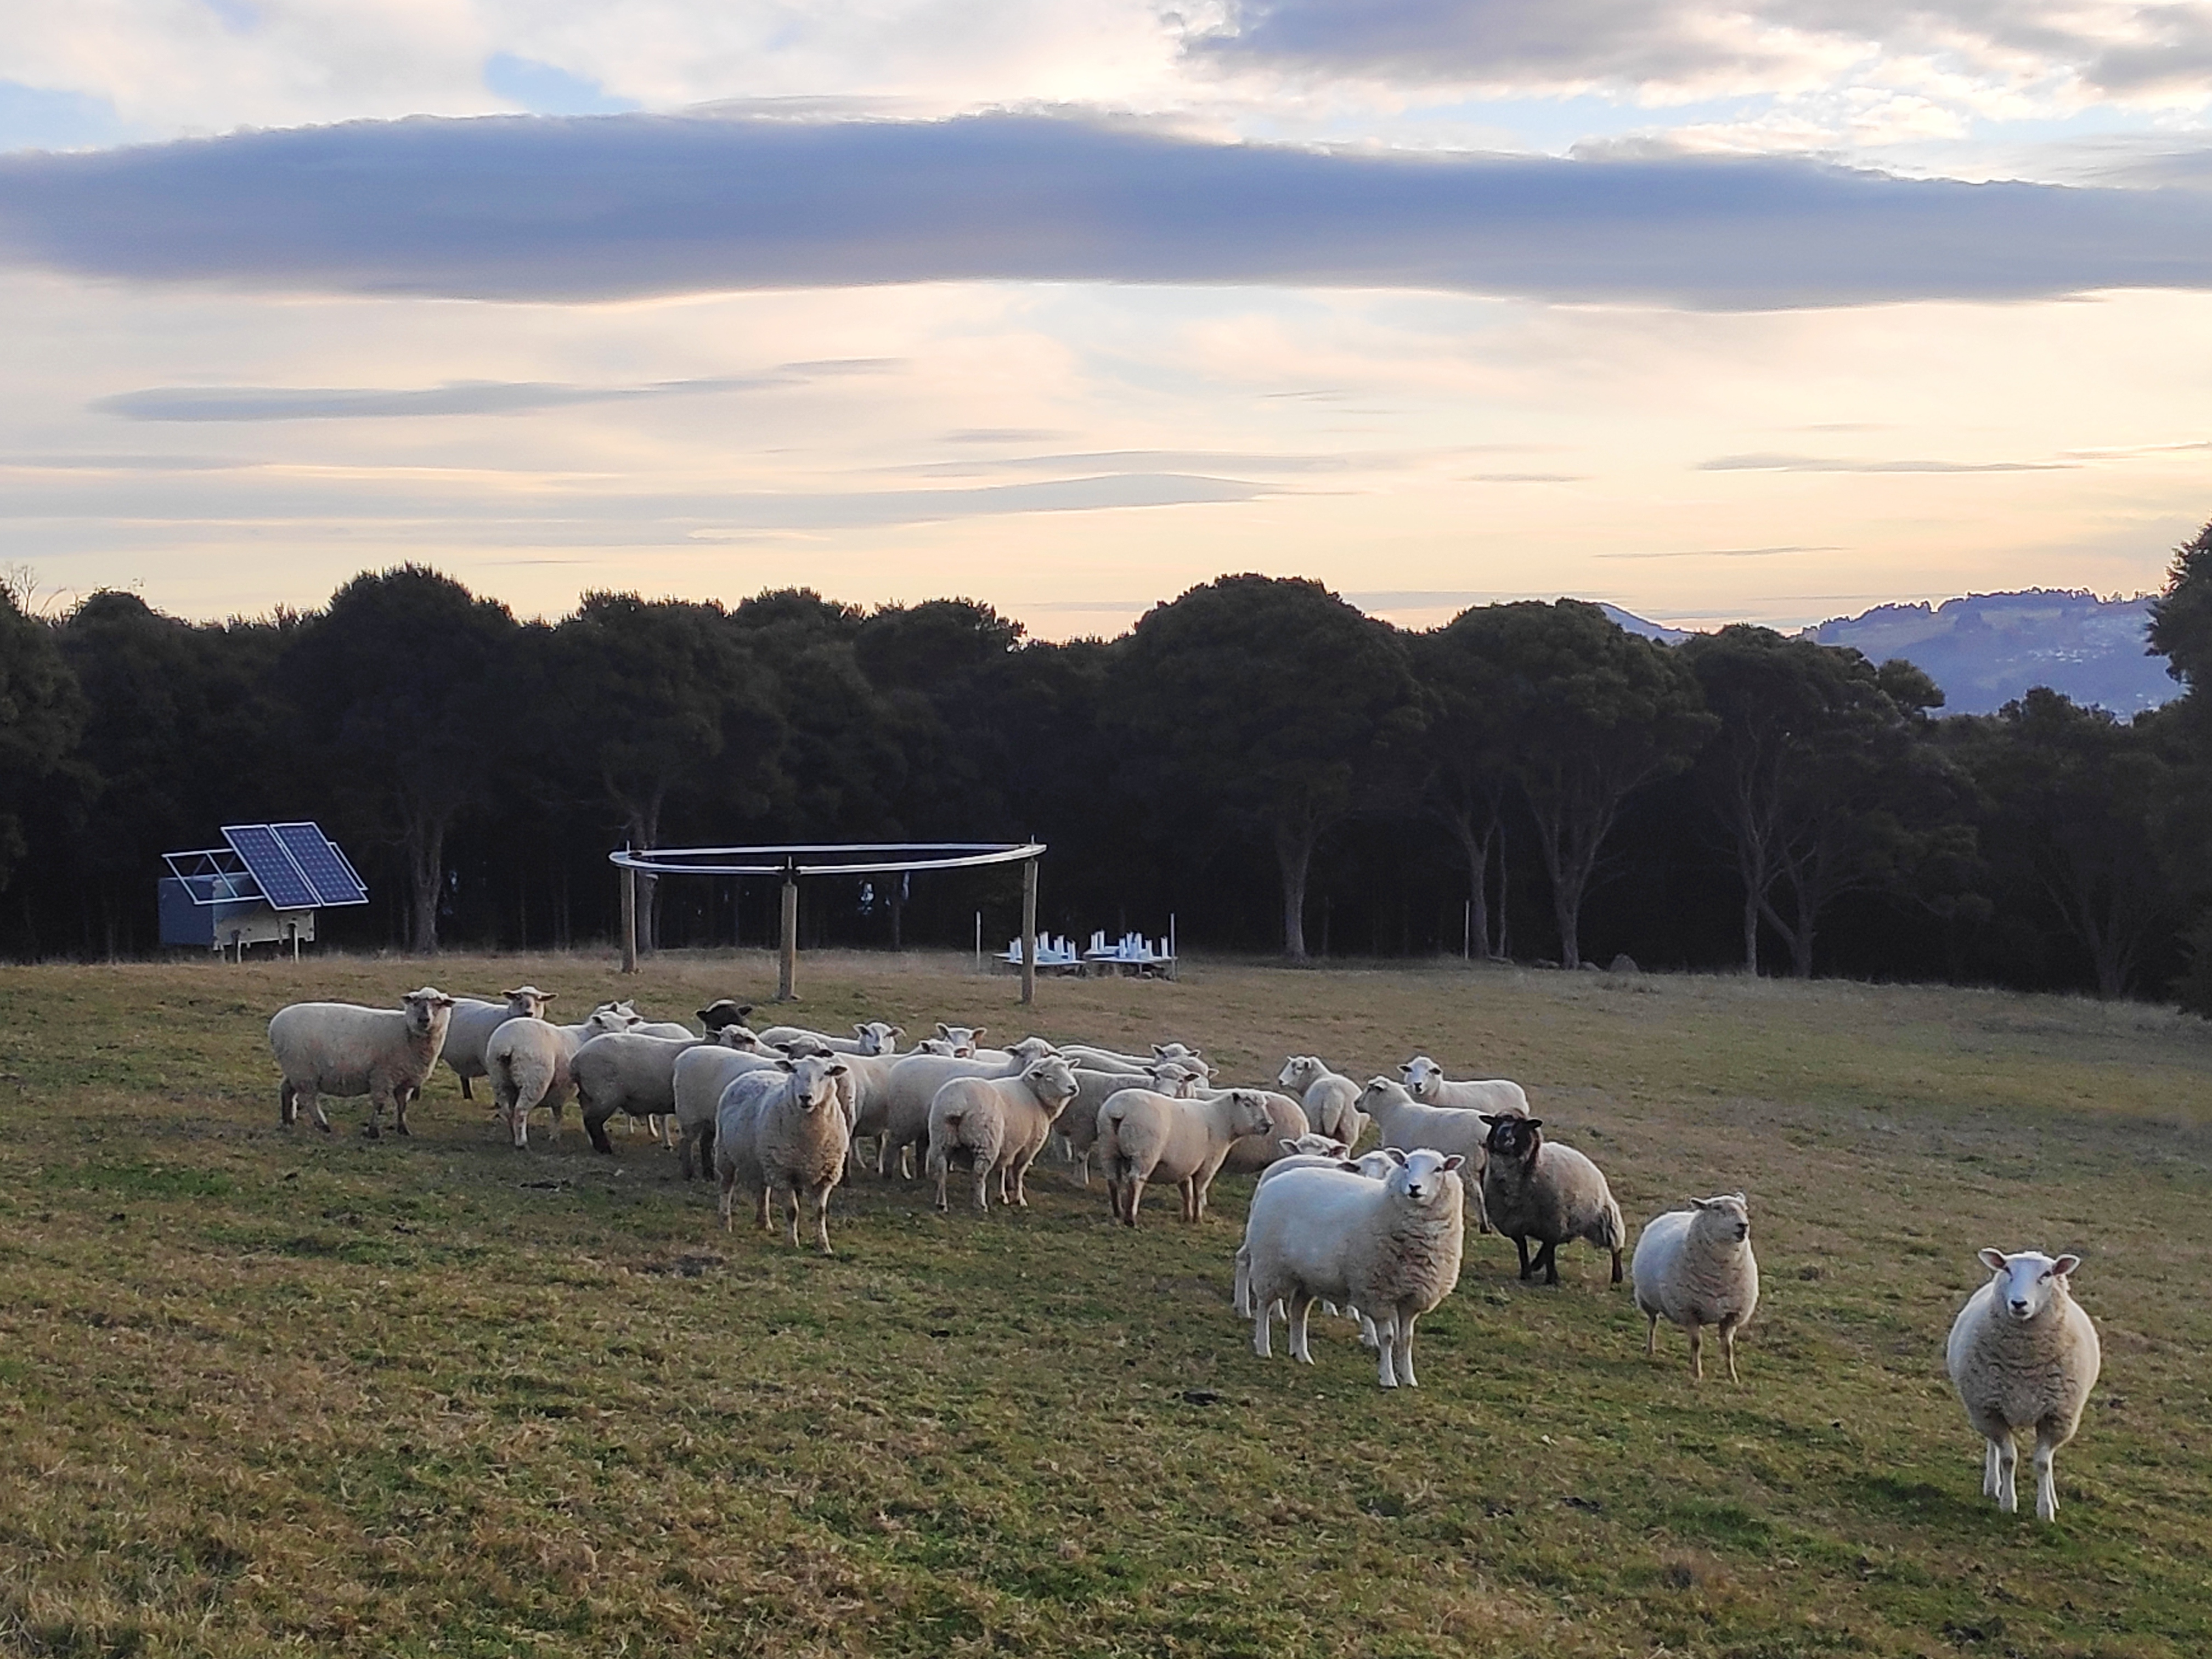
\includegraphics[width=\linewidth]{../tart_calibration/fig/radio_agronomy.jpg}
\end{frame}


\begin{frame}[allowframebreaks]
    \frametitle{References}
    \bibliographystyle{amsalpha}
    \bibliography{array_design.bib}
\end{frame}

\end{document}
